\documentclass[a4paper, 12pt]{article}
\usepackage[utf8x]{inputenc}
\usepackage{cmap}
\usepackage[english, russian]{babel}
\usepackage{indentfirst}
\usepackage[left=20mm, top=20mm, right=20mm, bottom=20mm]{geometry}
\usepackage{tikz}
\usepackage{float}
\usepackage{amsmath, amsfonts, amssymb}
\usepackage{graphicx}
\usepackage{fancybox, fancyhdr}
\usepackage{hyperref}
\usepackage{listings}
\usepackage{caption}
\usepackage{subcaption}
\usepackage{xcolor}
\pagestyle{fancy}
\fancyhf{}
\fancyhead[L]{Лабораторная работа №3}
\fancyhead[R]{Частотные методы}
\fancyfoot[C]{\thepage}
\graphicspath{{images/}}
\usetikzlibrary{patterns}
\definecolor{LightGray}{gray}{0.95}
\lstdefinestyle{pycode}{
    language=Python,
    basicstyle=\footnotesize\ttfamily,
    numbers=left,
    numberstyle=\tiny\color{gray},
    stepnumber=1,
    numbersep=5pt,
    backgroundcolor=\color{LightGray},
    showspaces=false,
    showstringspaces=false,
    showtabs=false,
    tabsize=4,
    captionpos=b,
    breaklines=true,
    breakatwhitespace=false,
    frame=none,
    rulecolor=\color{black},
    linewidth=\linewidth,
    keywordstyle=\color{red}\bfseries,
    commentstyle=\color{green!40!black},
    stringstyle=\color{blue},
    escapeinside={\%*}{*)},
    xleftmargin=0pt,
    framexleftmargin=0pt,
    framexrightmargin=0pt
}
\lstset{style=pycode}
\hypersetup{
    colorlinks=true,
    linkcolor=blue,
    filecolor=magenta,      
    urlcolor=cyan,
    pdftitle={contents setup},
    pdfpagemode=FullScreen,
}
\setlength{\parskip}{1.5mm}
\setlength{\headheight}{15pt}
\setlength{\footskip}{15pt}
\allowdisplaybreaks
\DeclareMathOperator{\sinc}{sinc}
\newcommand{\frc}[2]{\raisebox{2pt}{$#1$}\big/\raisebox{-3pt}{$#2$}}

\begin{document}
    \begin{titlepage}

        \begin{center}
        
\includegraphics[width=0.3\textwidth]{itmo.png} % requires itmo.png in /images folder
        \vfill
        
        Федеральное государственное автономное образовательное учреждение высшего образования
        «Национальный Исследовательский Университет ИТМО»\\
        
        \vfill
        {\large\bf ЛАБОРАТОРНАЯ РАБОТА №3}\\
        {\large\bf ПРЕДМЕТ «ЧАСТОТНЫЕ МЕТОДЫ»}\\
        {\large\bf ТЕМА «ЖЕСТКАЯ ФИЛЬТРАЦИЯ»}
        \vfill

        \begin{flushright}
            \begin{minipage}{.45\textwidth}
            {
                \hbox{Лектор: Перегудин А. А.}
                \hbox{Практик: Пашенко А. В.}
                \hbox{Студент: Румянцев А. А.}
                \hbox{Поток: ЧАСТ.МЕТ. 1.3}
                \hbox{}
                \hbox{Факультет: СУиР}
                \hbox{Группа: R3241}
            }
            \end{minipage}
        \end{flushright}
        
        \vfill
                
        Санкт-Петербург\\
        2024
        \end{center}
    \end{titlepage}
    
    \tableofcontents

    \newpage
% \end{document}
    \section{Задание 1. Жесткие фильтры}
    Зададим такие числа $a,\,t_1,\,t_2$, что $t_1<t_2$, и рассмотрим функцию $g$ такую, что
    $g(t)=a$ при $t\in[t_1,t_2]$ и $g(t)=0$ при других $t$. $$\sqsupset a=2,\ \ t_1=-1.5,\ \ t_2=2.5,\ \ g(t)=
    \begin{cases}
        2, & t\in[t_1,t_2]\\
        0, & \text{ otherwise}
    \end{cases}
    $$


    Выберем интервал времени $T=10$ и шаг дискретизации $dt=0.01$. Зададим в python массив времени $t$ от $-0.5\cdot T$ до $0.5\cdot T+dt$
    с шагом $dt$ и включим последнюю точку. Найдем список значений $g$ и зададим зашумленную версию сигнала как
    $$
    u=g+b\cdot(\text{random}(\text{len}(t))-0.5) + c\cdot \sin(d\cdot t);
    $$


    В данном задании мы выполняем жесткую фильтрацию сигнала $u$. Алгоритм следующий: находится Фурье-образ от сигнала,
    обнуляются его значения на некоторых диапазонах частот, затем сигнал восстанавливается обратным преобразованием Фурье.
    Далее строятся графики с помощью программы на языке python. Используемый код с пояснениями находится в отдельной секции.


    В задаваемом сигнале параметр $a$ отвечает за высоту, на которую поднимется часть сигнала от нуля, а $t_1 \text{ и } t_2$ -- начало
    и конец промежутка с подъемом соответственно. Таким образом, на интервале длины $t_2-t_1=2.5+1.5=4$, начиная с $t_1=-1.5$ и заканчивая $t_2=2.5$,
    на высоте $a=2$ будет находится часть от всего сигнала, который, в свою очередь, располагается на промежутке $[-0.5\cdot T,0.5\cdot T]=[-5,5]$
    длины $2\cdot T\cdot 0.5=10$. Параметры $b,\,c,\,d$ отвечают за шум, присутствующий в сигнале. Далее будут рассмотрены графики и сделаны выводы о
    влиянии каждого параметра на сам сигнал и на его результат фильтрации.


    \subsection{Убираем высокие частоты. Фильтр нижних частот}
    Возьмем параметр $c=0$. Далее действуем в соответствии с алгоритмом. Возьмем некоторый диапазон частот $[-\nu_0, \nu_0]$, на котором оставим Фурье-образ
    сигнала $u$ неизменным, а на остальных частотах обнулим его значения. Такое поведение соответствует фильтру \textit{нижних} частот, так как он пропускает
    все частоты ниже частоты среза. Построим сравнительные графики исходного и фильтрованного сигналов на некотором интервале $[t_1,t_2]$, а также модуля
    Фурье-образа исходного и фильтрованного сигналов. Исследуем влияние частоты среза $\nu_0$ и значения параметра $b$ на эффективность фильтрации.
    
    
    Далее будут приведены рисунки полученных графиков. На каждом графике подписаны выбранные значения $b,\,c,\,d,\,\nu_0$
    (хотя, при условии, что $c=0$, менять или рассматривать параметр $d$ не требуется). Также отмечена легенда -- синим цветом
    обозначается оригинальный сигнал, красным фильтрованный.


    \begin{figure}[!htb]
        \centering
        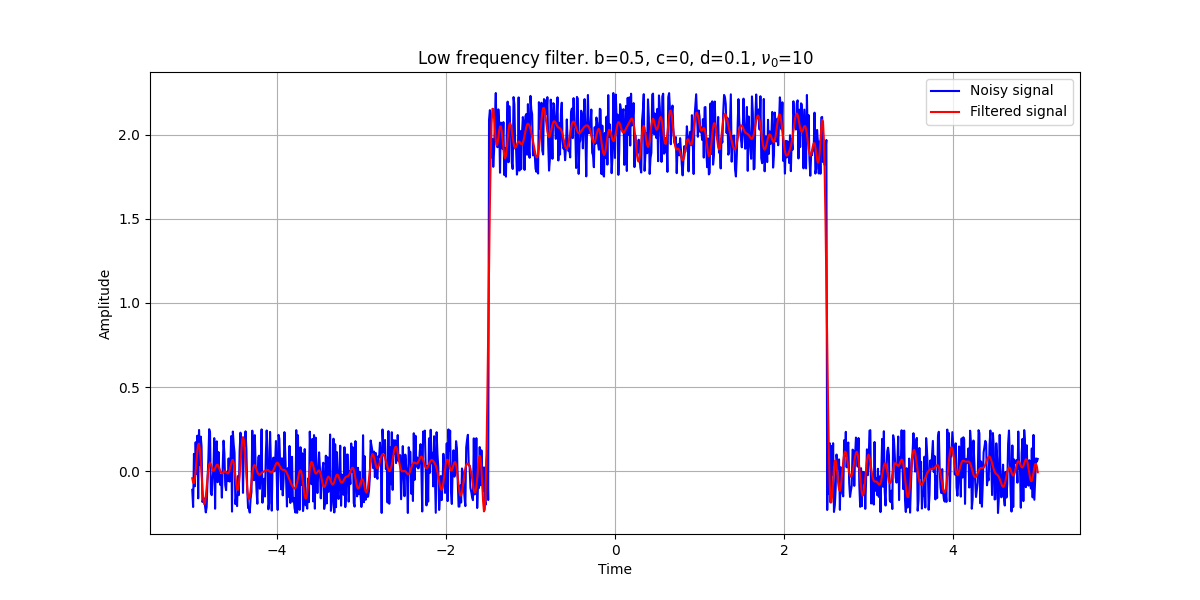
\includegraphics[scale=0.48]{1_u_flt_u_nohigh.png}
        \captionsetup{skip=0pt}
        \caption{График исходного и фильтрованного сигналов (1)}
        \label{fig:fig1}
    \end{figure}
    \begin{figure}[!htb]
        \centering
        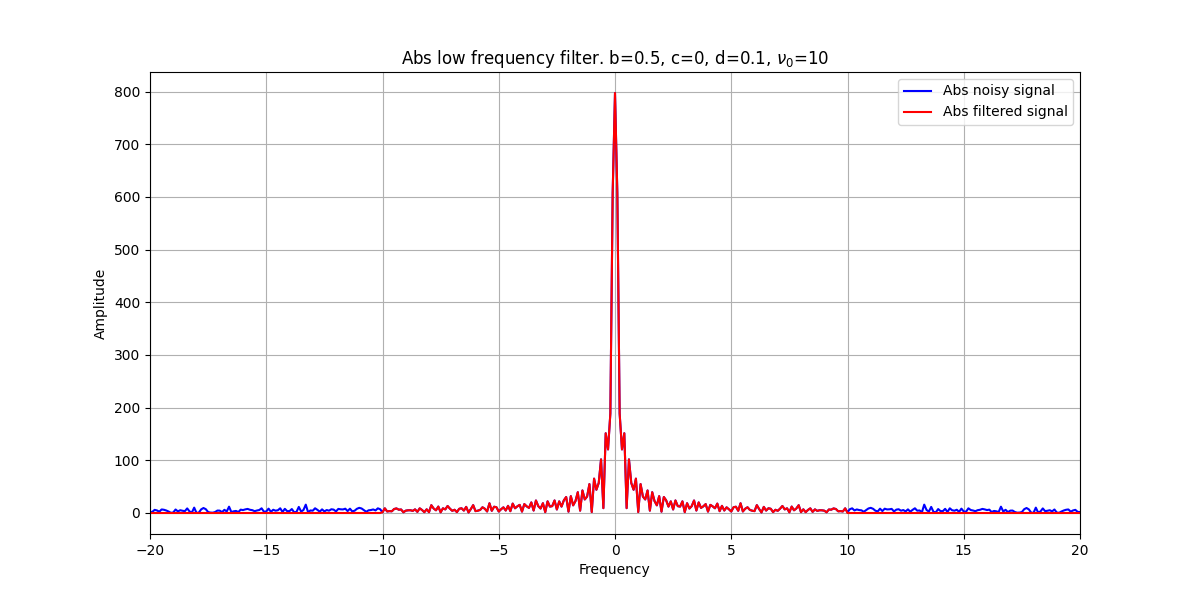
\includegraphics[scale=0.48]{1_abs_u_U_nohigh.png}
        \captionsetup{skip=0pt}
        \caption{График модуля Фурье-образа исходного и фильтрованного сигналов (1)}
        \label{fig:fig2}
    \end{figure}
    \begin{figure}[!htb]
        \centering
        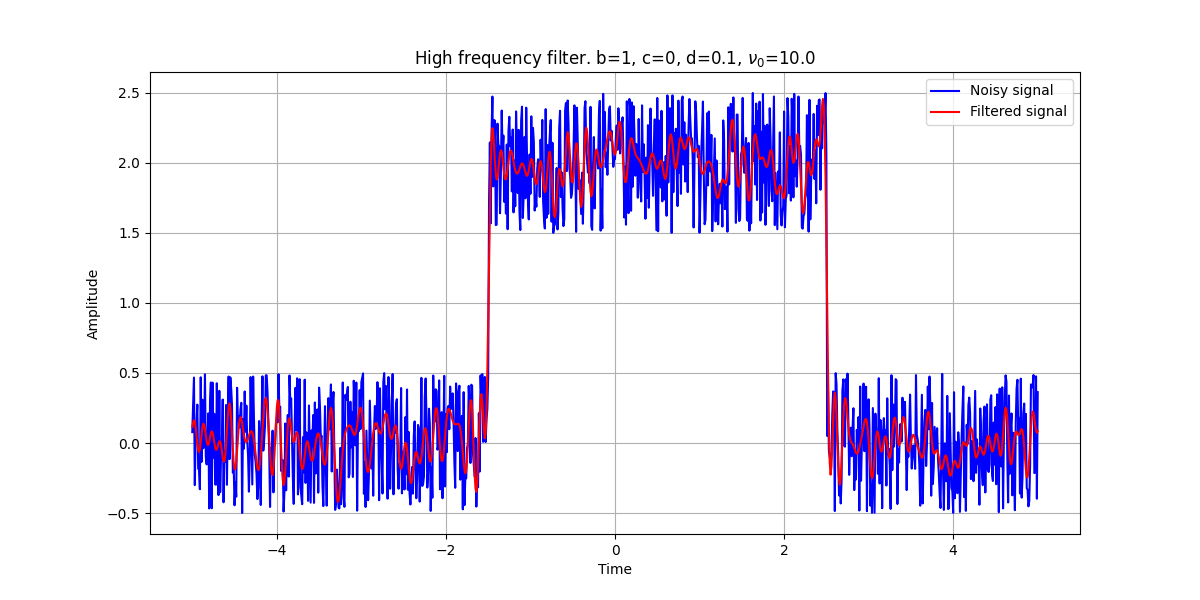
\includegraphics[scale=0.48]{2_u_flt_u_nohigh.png}
        \captionsetup{skip=0pt}
        \caption{График исходного и фильтрованного сигналов (2)}
        \label{fig:fig3}
    \end{figure}
    \begin{figure}[!htb]
        \centering
        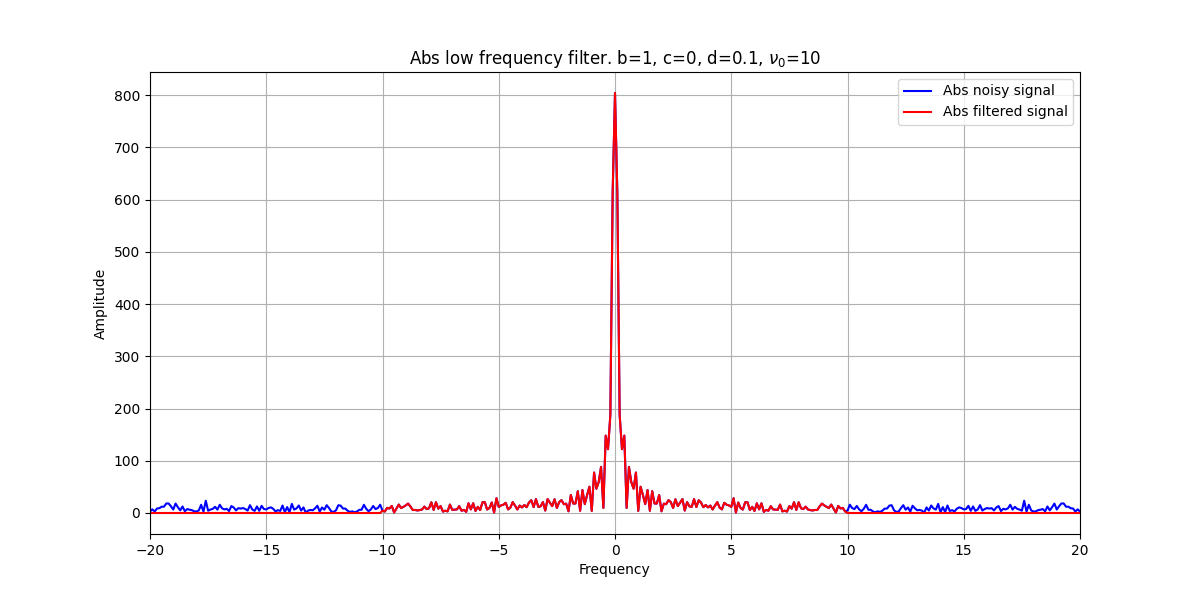
\includegraphics[scale=0.48]{2_abs_u_U_nohigh.png}
        \captionsetup{skip=0pt}
        \caption{График модуля Фурье-образа исходного и фильтрованного сигналов (2)}
        \label{fig:fig4}
    \end{figure}
    \begin{figure}[!htb]
        \centering
        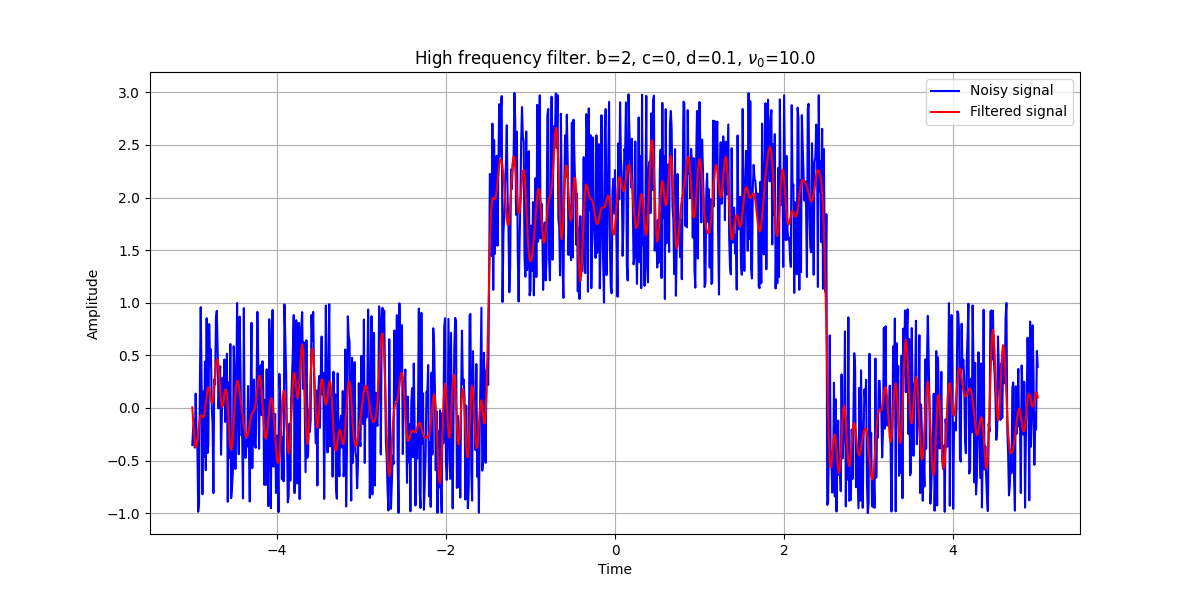
\includegraphics[scale=0.48]{3_u_flt_u_nohigh.png}
        \captionsetup{skip=0pt}
        \caption{График исходного и фильтрованного сигналов (3)}
        \label{fig:fig5}
    \end{figure}
    \begin{figure}[!htb]
        \centering
        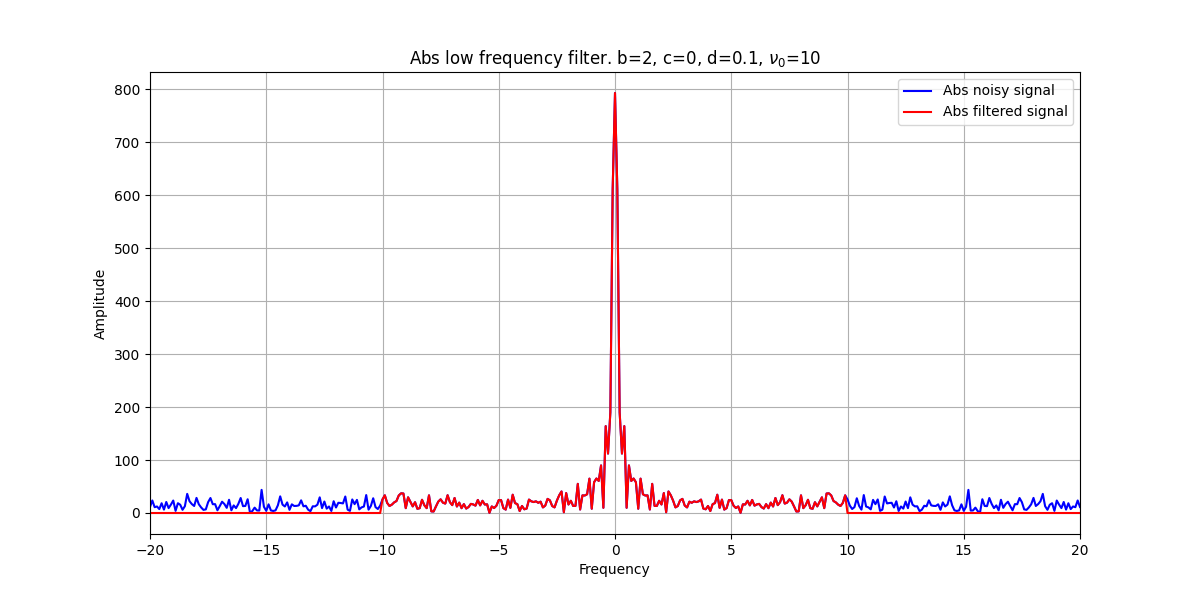
\includegraphics[scale=0.48]{3_abs_u_U_nohigh.png}
        \captionsetup{skip=0pt}
        \caption{График модуля Фурье-образа исходного и фильтрованного сигналов (3)}
        \label{fig:fig6}
    \end{figure}
    \begin{figure}[!htb]
        \centering
        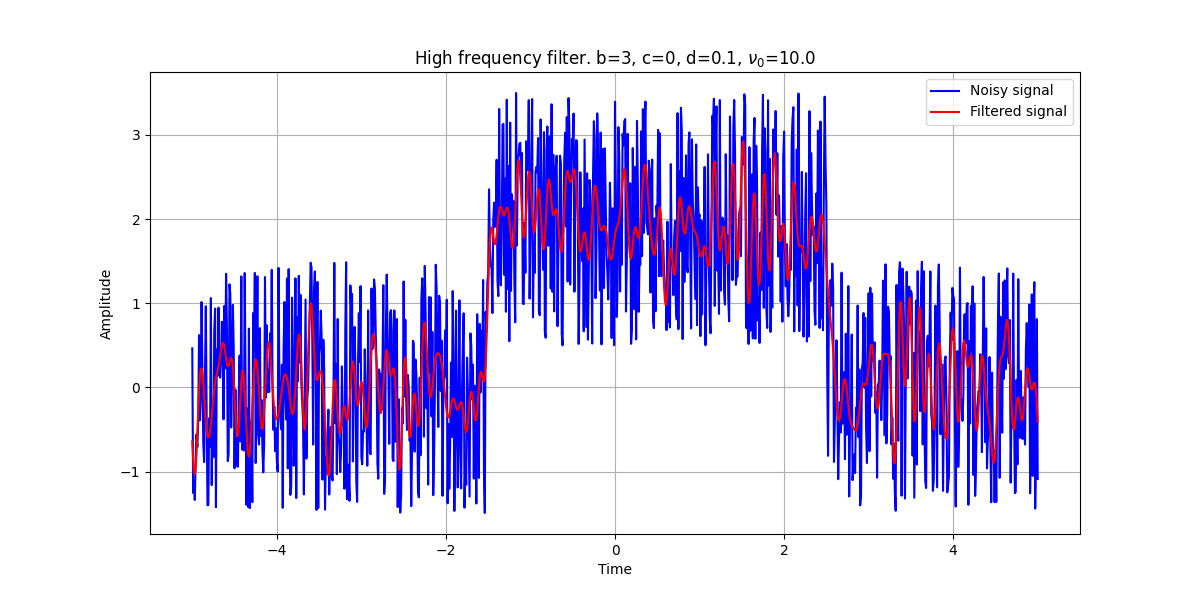
\includegraphics[scale=0.48]{5_u_flt_u_nohigh.png}
        \captionsetup{skip=0pt}
        \caption{График исходного и фильтрованного сигналов (4)}
        \label{fig:fig7}
    \end{figure}
    \begin{figure}[!htb]
        \centering
        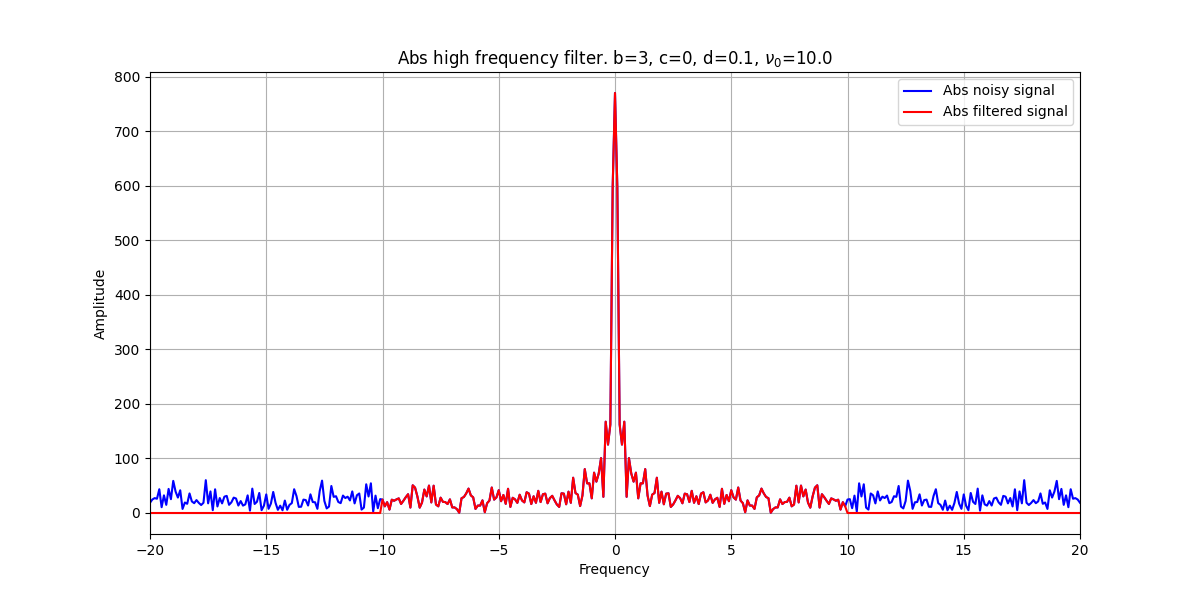
\includegraphics[scale=0.48]{5_abs_u_U_nohigh.png}
        \captionsetup{skip=0pt}
        \caption{График модуля Фурье-образа исходного и фильтрованного сигналов (4)}
        \label{fig:fig8}
    \end{figure}
    \begin{figure}[!htb]
        \centering
        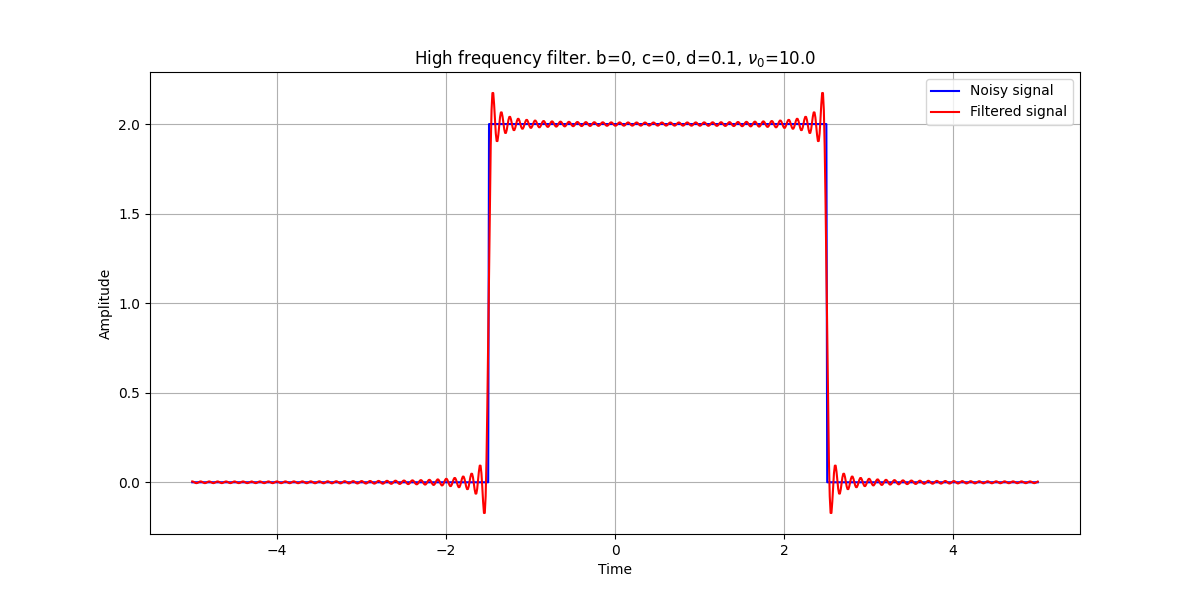
\includegraphics[scale=0.48]{4_u_flt_u_nohigh.png}
        \captionsetup{skip=0pt}
        \caption{График исходного и фильтрованного сигналов (5)}
        \label{fig:fig9}
    \end{figure}
    \begin{figure}[!htb]
        \centering
        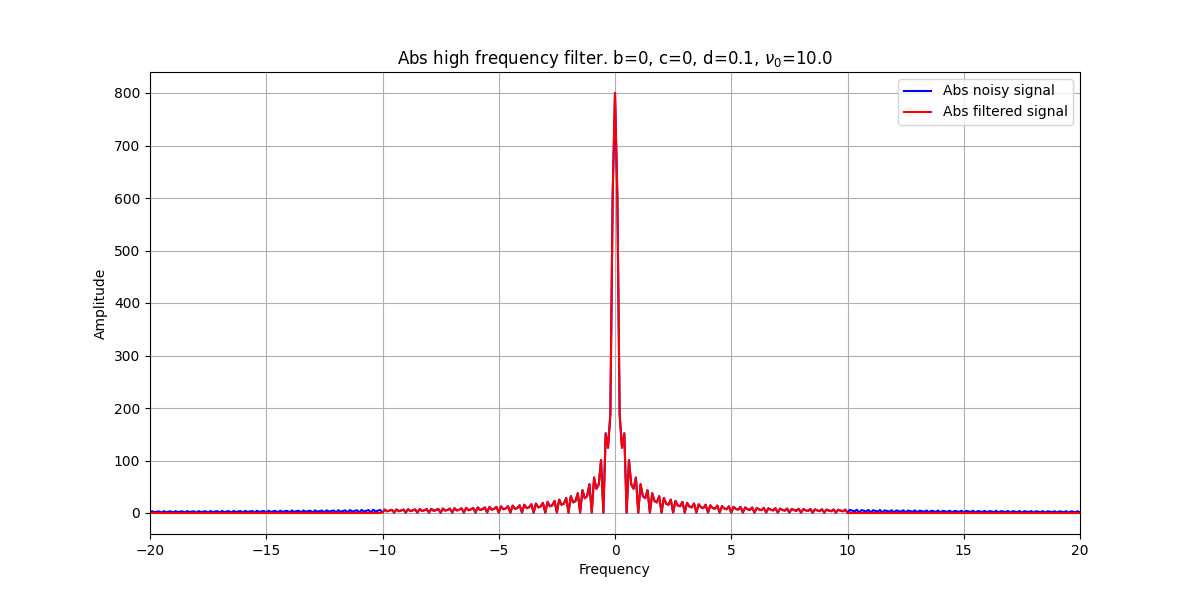
\includegraphics[scale=0.48]{4_abs_u_U_nohigh.png}
        \captionsetup{skip=0pt}
        \caption{График модуля Фурье-образа исходного и фильтрованного сигналов (5)}
        \label{fig:fig10}
    \end{figure}
    \begin{figure}[!htb]
        \centering
        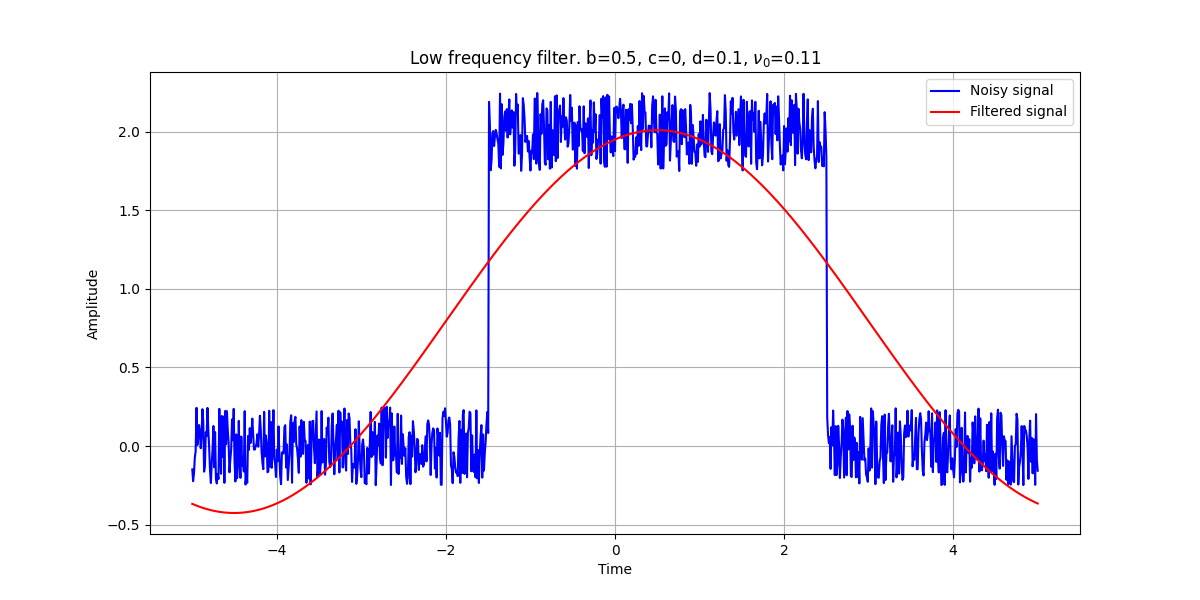
\includegraphics[scale=0.48]{11_u_flt_u_nohigh.png}
        \captionsetup{skip=0pt}
        \caption{График исходного и фильтрованного сигналов (6)}
        \label{fig:fig11}
    \end{figure}
    \begin{figure}[!htb]
        \centering
        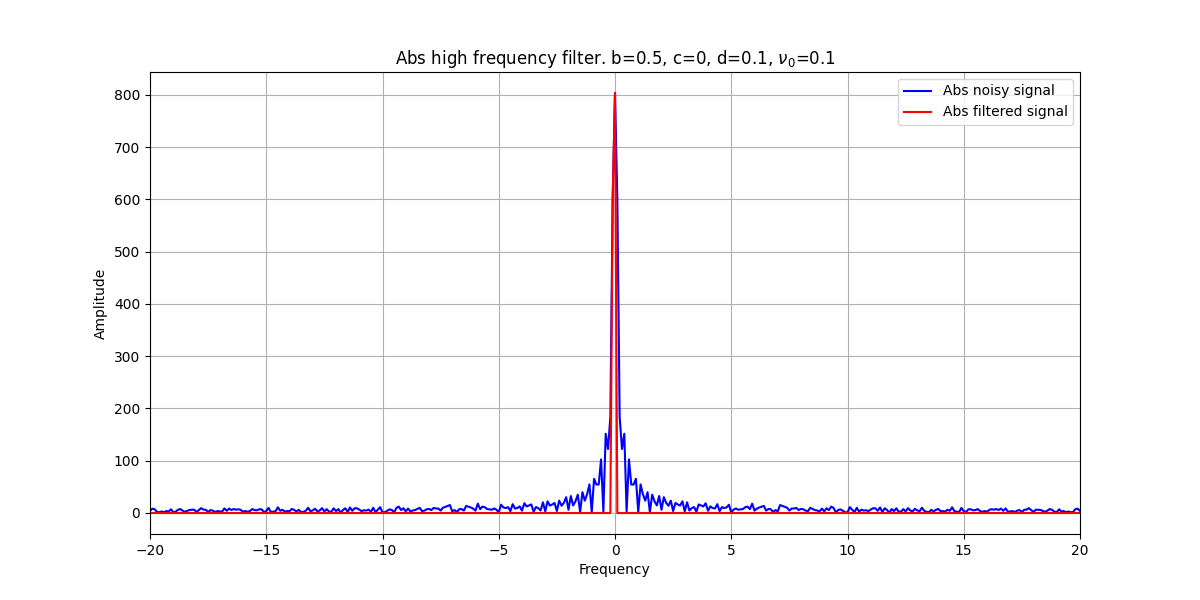
\includegraphics[scale=0.48]{11_abs_u_U_nohigh.png}
        \captionsetup{skip=0pt}
        \caption{График модуля Фурье-образа исходного и фильтрованного сигналов (6)}
        \label{fig:fig12}
    \end{figure}
    \begin{figure}[!htb]
        \centering
        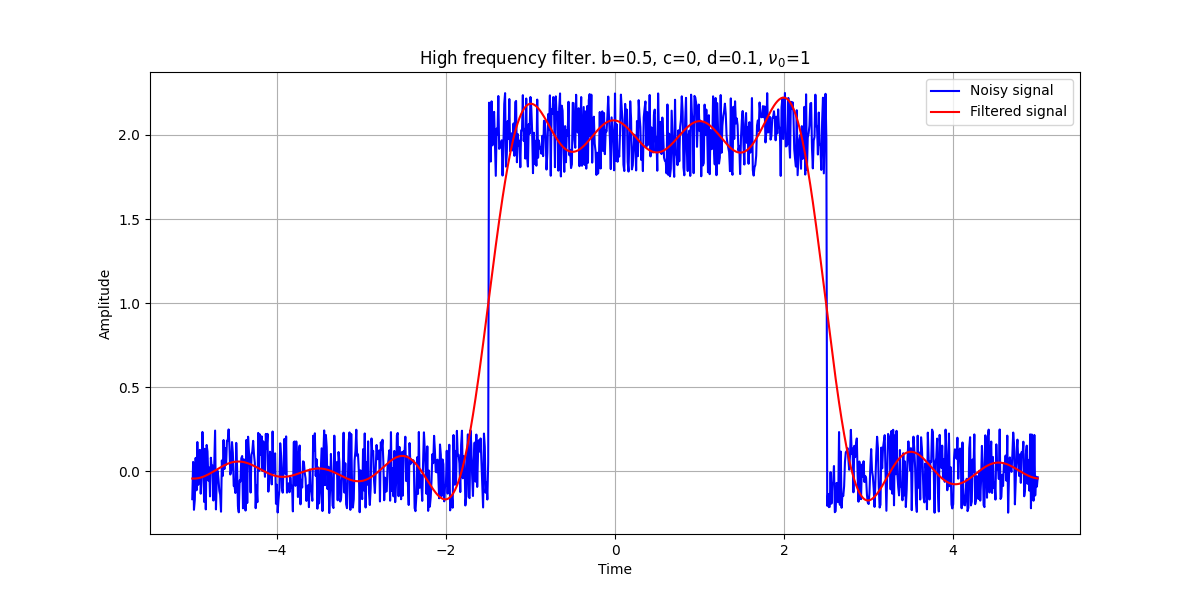
\includegraphics[scale=0.48]{12_u_flt_u_nohigh.png}
        \captionsetup{skip=0pt}
        \caption{График исходного и фильтрованного сигналов (7)}
        \label{fig:fig13}
    \end{figure}
    \begin{figure}[!htb]
        \centering
        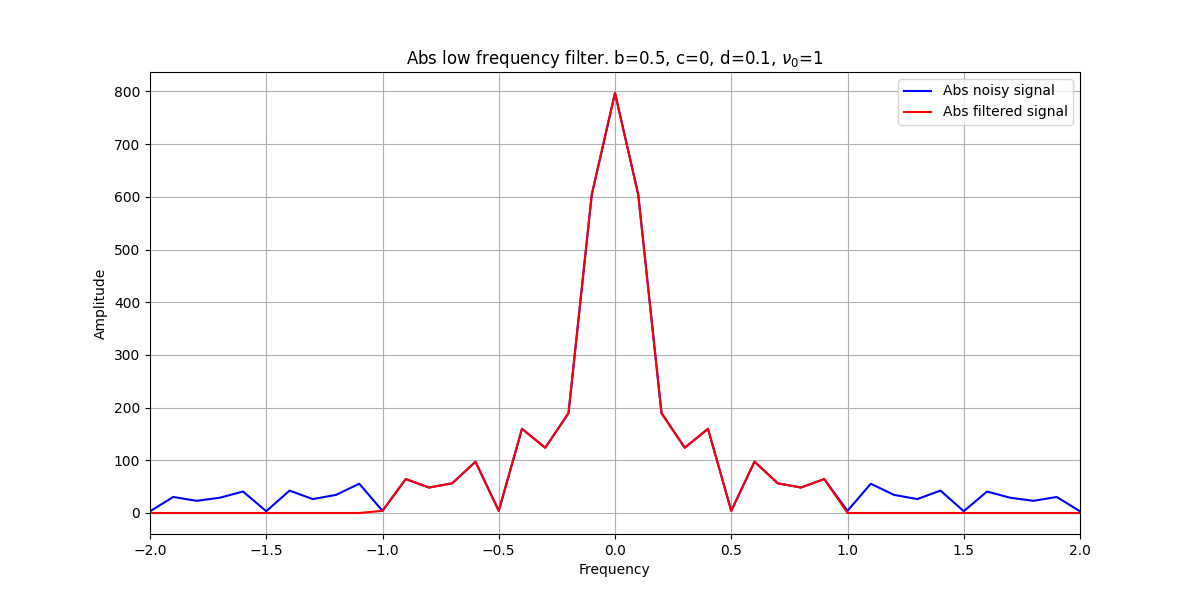
\includegraphics[scale=0.48]{12_abs_u_U_nohigh.png}
        \captionsetup{skip=0pt}
        \caption{График модуля Фурье-образа исходного и фильтрованного сигналов (7)}
        \label{fig:fig14}
    \end{figure}
    \begin{figure}[!htb]
        \centering
        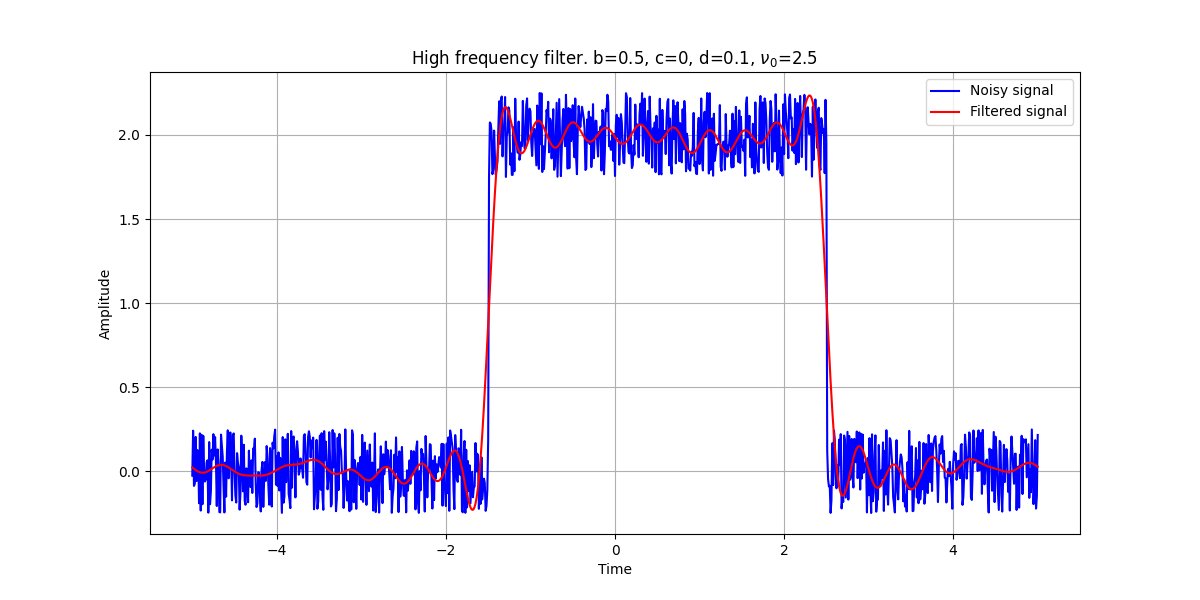
\includegraphics[scale=0.48]{13_u_flt_u_nohigh.png}
        \captionsetup{skip=0pt}
        \caption{График исходного и фильтрованного сигналов (8)}
        \label{fig:fig15}
    \end{figure}
    \begin{figure}[!htb]
        \centering
        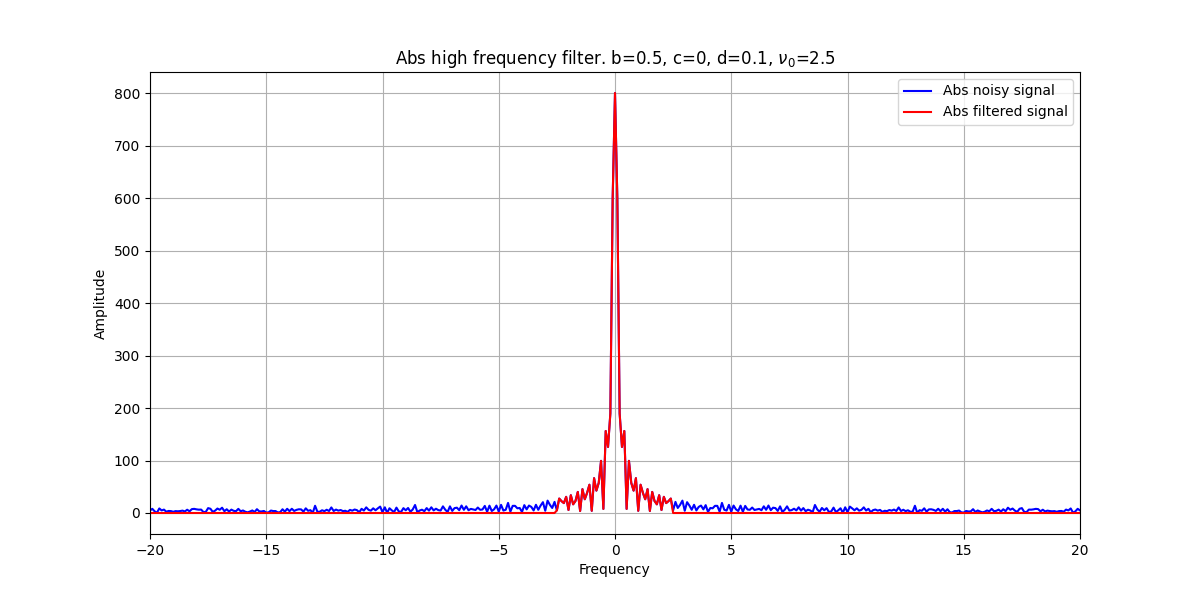
\includegraphics[scale=0.48]{13_abs_u_U_nohigh.png}
        \captionsetup{skip=0pt}
        \caption{График модуля Фурье-образа исходного и фильтрованного сигналов (8)}
        \label{fig:fig16}
    \end{figure}
    \begin{figure}[!htb]
        \centering
        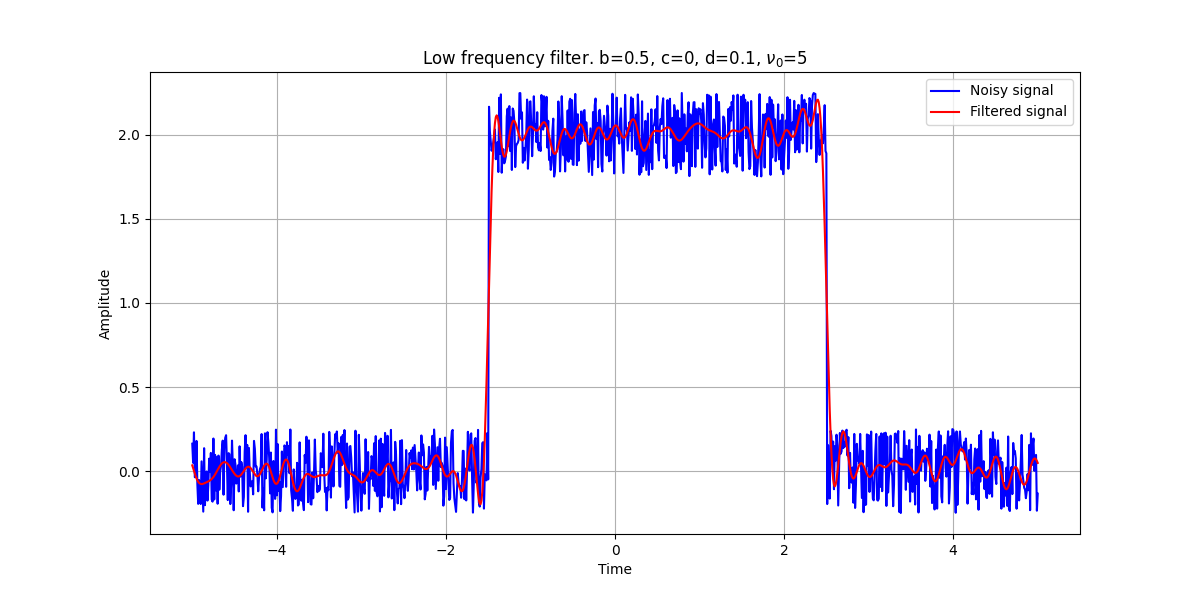
\includegraphics[scale=0.48]{8_u_flt_u_nohigh.png}
        \captionsetup{skip=0pt}
        \caption{График исходного и фильтрованного сигналов (9)}
        \label{fig:fig17}
    \end{figure}
    \begin{figure}[!htb]
        \centering
        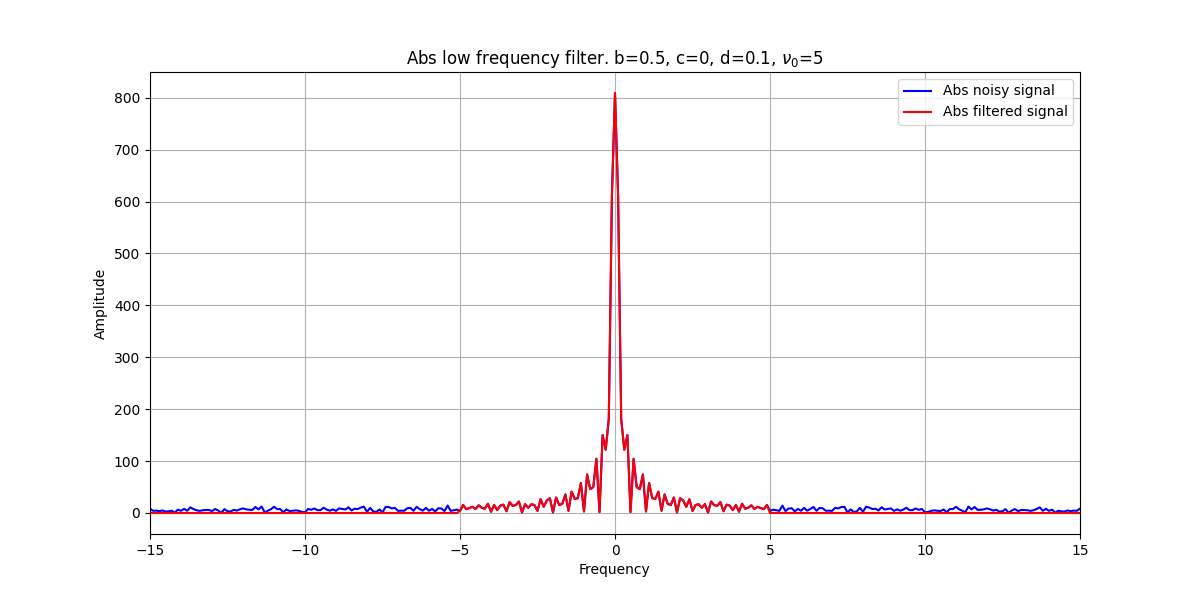
\includegraphics[scale=0.48]{8_abs_u_U_nohigh.png}
        \captionsetup{skip=0pt}
        \caption{График модуля Фурье-образа исходного и фильтрованного сигналов (9)}
        \label{fig:fig18}
    \end{figure}
    \begin{figure}[!htb]
        \centering
        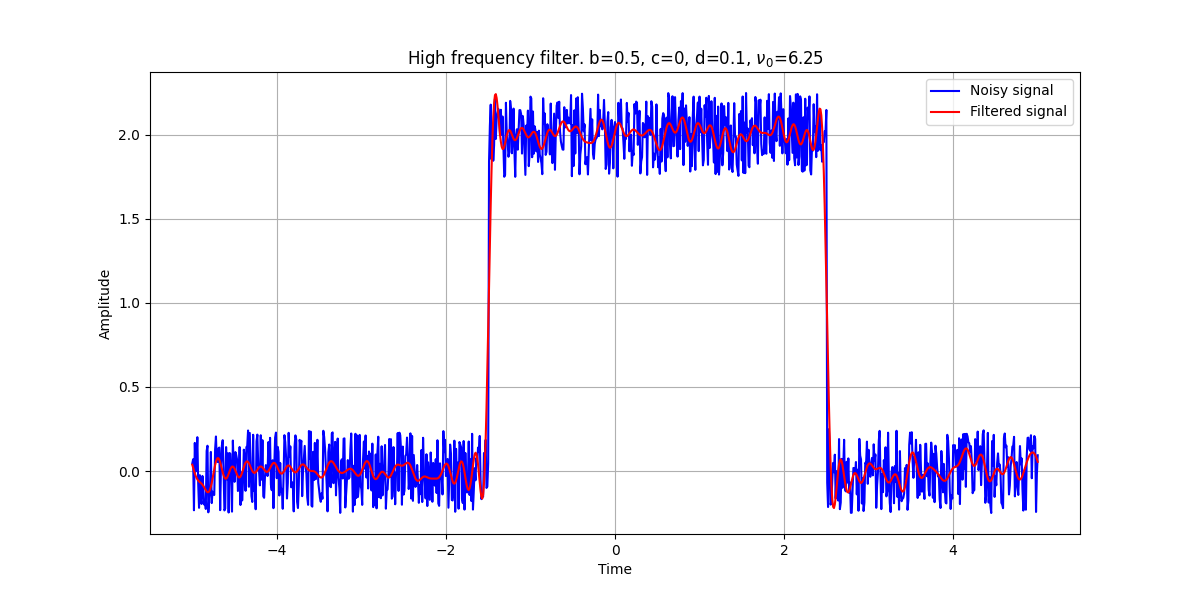
\includegraphics[scale=0.48]{7_u_flt_u_nohigh.png}
        \captionsetup{skip=0pt}
        \caption{График исходного и фильтрованного сигналов (10)}
        \label{fig:fig19}
    \end{figure}
    \begin{figure}[!htb]
        \centering
        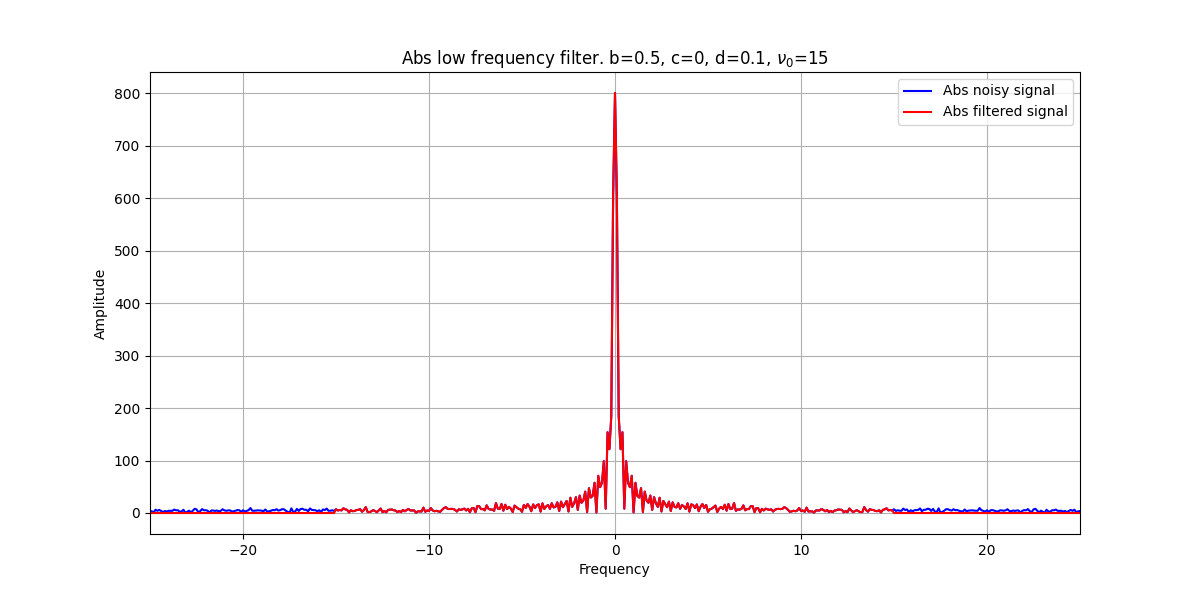
\includegraphics[scale=0.48]{7_abs_u_U_nohigh.png}
        \captionsetup{skip=0pt}
        \caption{График модуля Фурье-образа исходного и фильтрованного сигналов (10)}
        \label{fig:fig20}
    \end{figure}
    \begin{figure}[!htb]
        \centering
        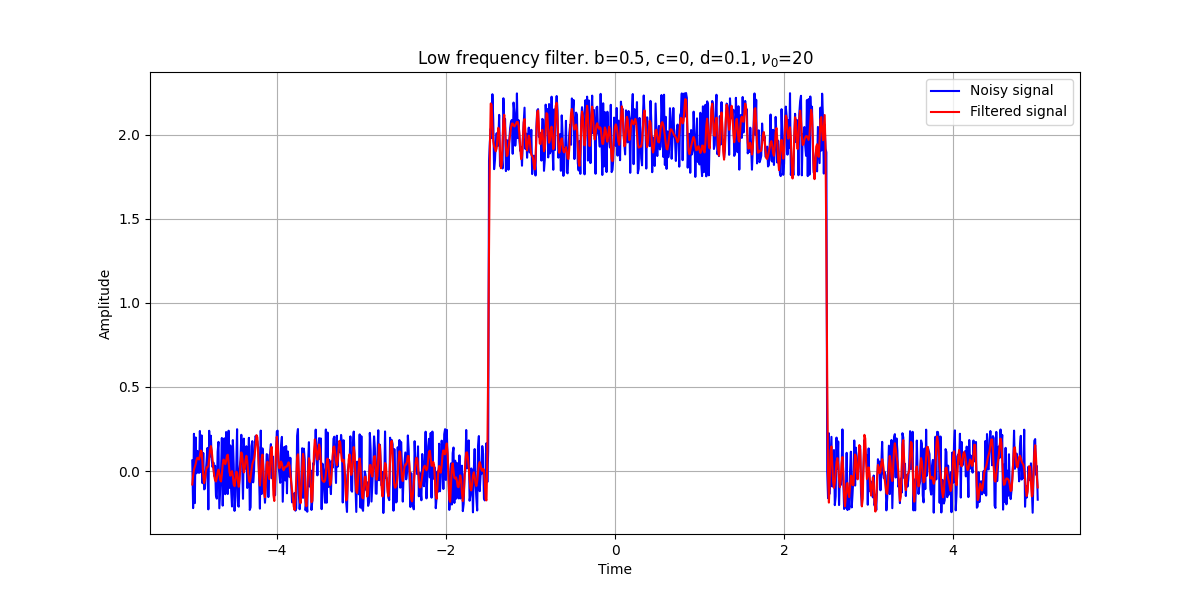
\includegraphics[scale=0.48]{6_u_flt_u_nohigh.png}
        \captionsetup{skip=0pt}
        \caption{График исходного и фильтрованного сигналов (11)}
        \label{fig:fig21}
    \end{figure}
    \begin{figure}[!htb]
        \centering
        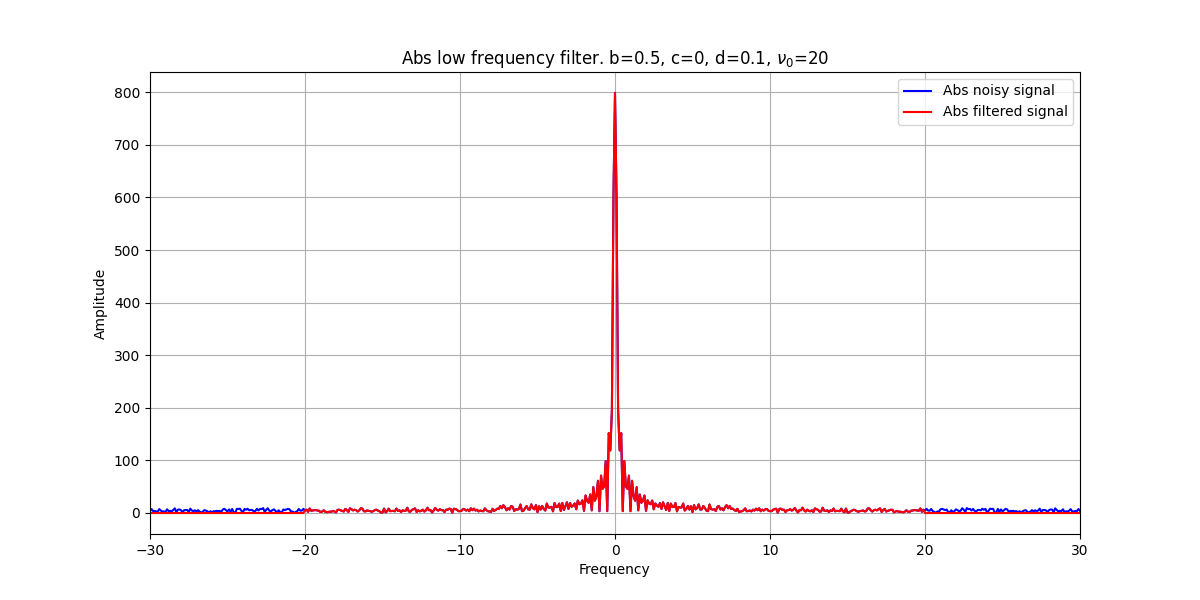
\includegraphics[scale=0.48]{6_abs_u_U_nohigh.png}
        \captionsetup{skip=0pt}
        \caption{График модуля Фурье-образа исходного и фильтрованного сигналов (11)}
        \label{fig:fig22}
    \end{figure}
    \begin{figure}[!htb]
        \centering
        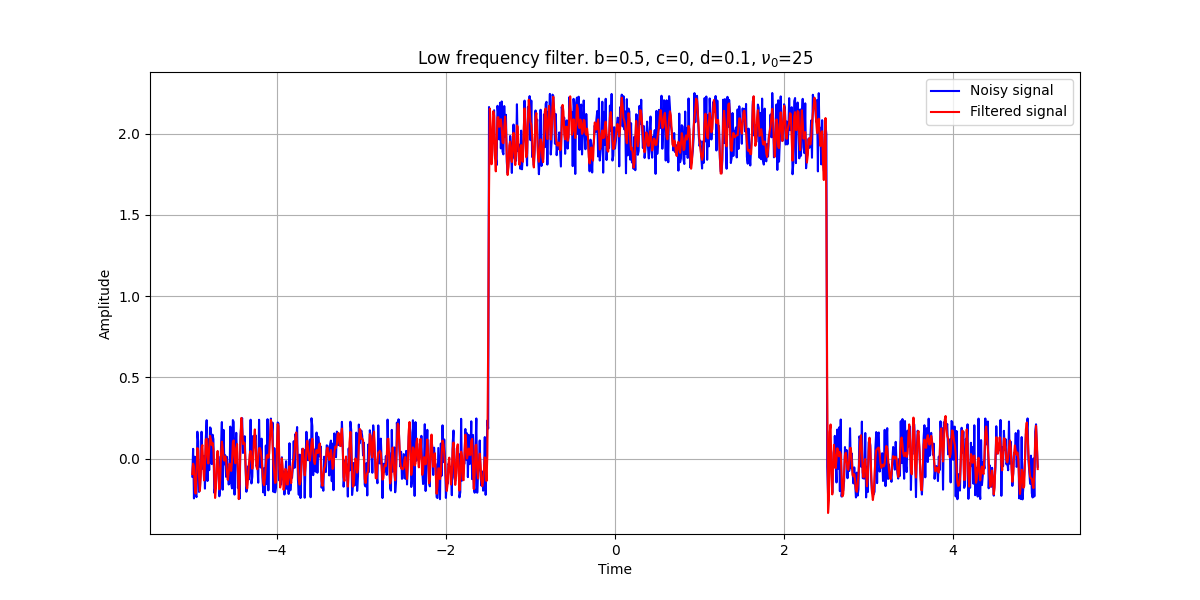
\includegraphics[scale=0.48]{10_u_flt_u_nohigh.png}
        \captionsetup{skip=0pt}
        \caption{График исходного и фильтрованного сигналов (12)}
        \label{fig:fig23}
    \end{figure}
    \begin{figure}[!htb]
        \centering
        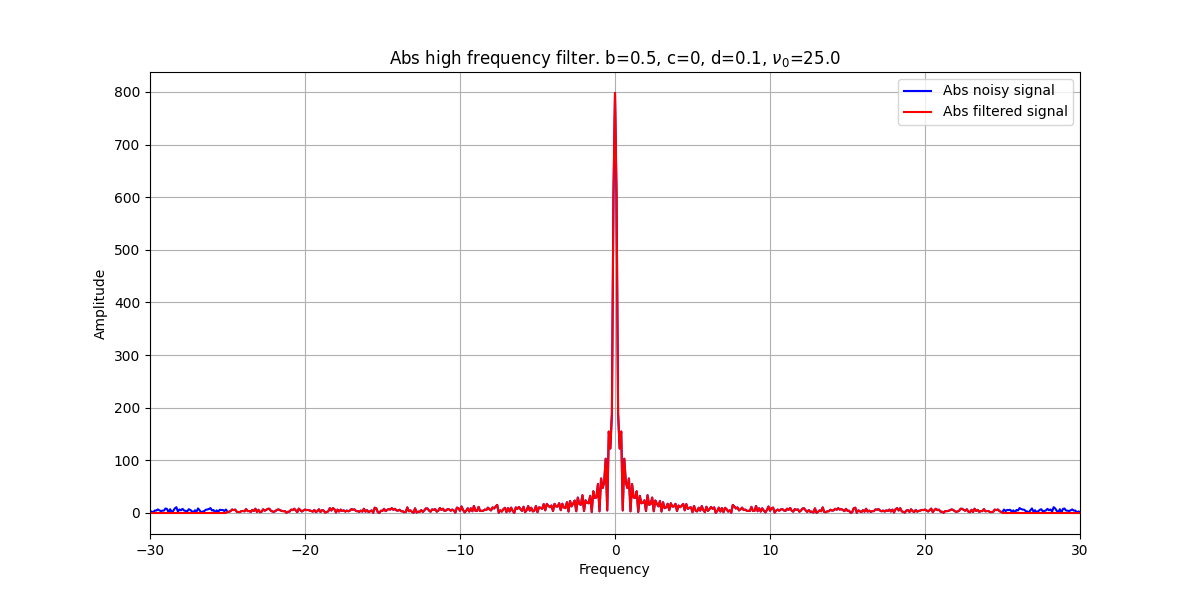
\includegraphics[scale=0.48]{10_abs_u_U_nohigh.png}
        \captionsetup{skip=0pt}
        \caption{График модуля Фурье-образа исходного и фильтрованного сигналов (12)}
        \label{fig:fig24}
    \end{figure}
    \begin{figure}[!htb]
        \centering
        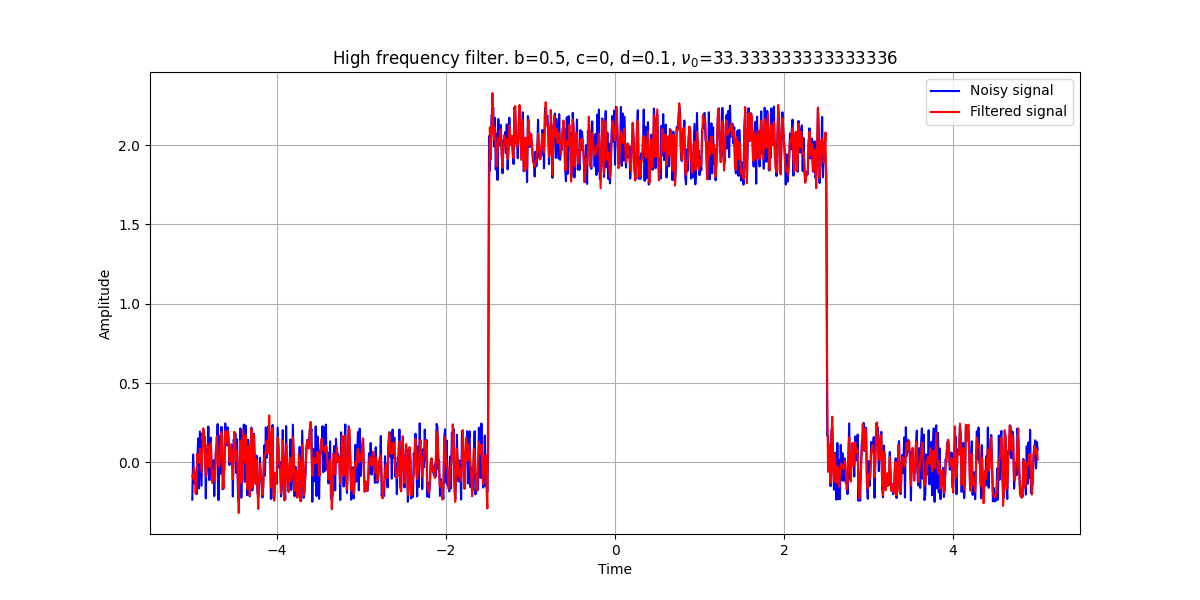
\includegraphics[scale=0.48]{9_u_flt_u_nohigh.png}
        \captionsetup{skip=0pt}
        \caption{График исходного и фильтрованного сигналов (13)}
        \label{fig:fig25}
    \end{figure}
    \begin{figure}[!htb]
        \centering
        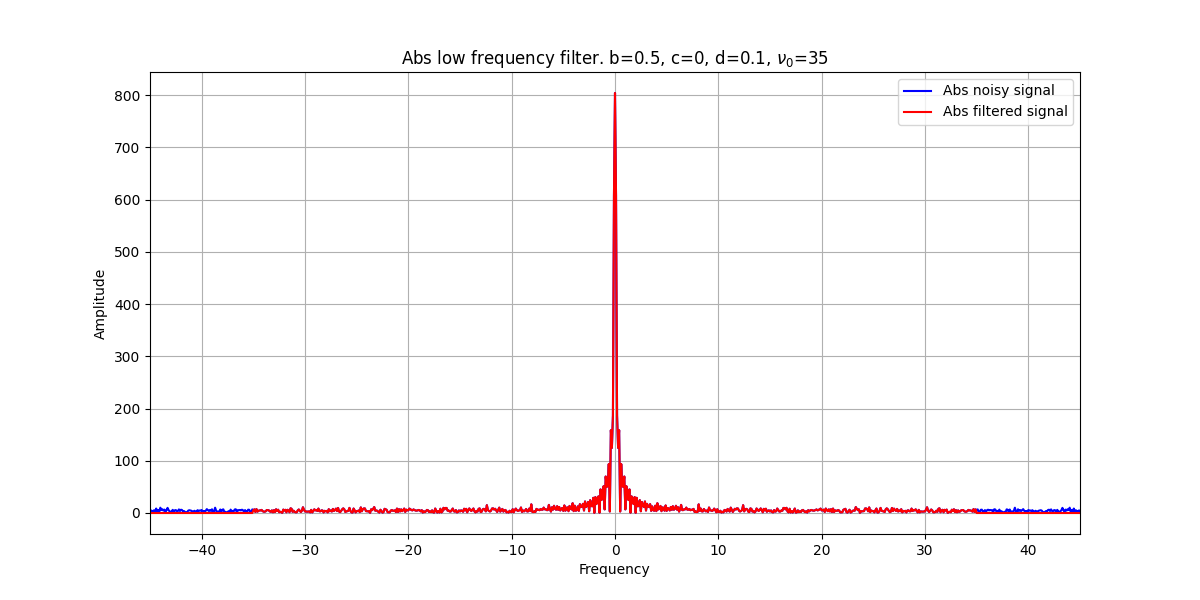
\includegraphics[scale=0.48]{9_abs_u_U_nohigh.png}
        \captionsetup{skip=0pt}
        \caption{График модуля Фурье-образа исходного и фильтрованного сигналов (13)}
        \label{fig:fig26}
    \end{figure}


    Исходя из графиков можно сделать вывод, что значение параметра $b$ отвечает за амплитуду каждой волны.
    Чем больше значение $b$, тем зашумленнее, <<грязнее>> выглядит сигнал, так как амплитуды волн возрастают.
    Фильтрованный сигнал при больших значениях $b$ также имеет более глубокие ямы и высокие подъемы, то есть
    испытывает увеличение амплитуды. Наглядно такое возрастание можно наблюдать на графиках модуля Фурье-образа
    исходного и фильтрованного сигналов -- на рисунке \ref{fig:fig2} амплитуды частот больше прижимаются к линии 
    $A=0$, а на рисунке \ref{fig:fig8} они больше стремятся к линии $A=50$, где $A$ -- амплитуда. Значение
    параметра $b$ влияет на эффективность фильтрации -- чем меньше значение $b$, тем чище сигнал и тем лучше
    фильтрация. При большом количестве белого шума фильтрация ухудшается (см. рис. \ref{fig:fig7}).
    При $b=0$ получается особый случай -- сигнал превращается в прямоугольную функцию, а фильтрованный
    сигнал выглядит как ее аппроксимация.


    Больше всего влияния на эффективность фильтрации оказывает частота среза $\nu_0$. Этот параметр необходимо подобрать
    так, чтобы оставались только те частоты, которые имеют заметно более высокую амплитуду по сравнению с остальными.
    Чем меньше частота среза $\nu_0$, тем заметно лучше фильтрация. Однако если взять слишком маленькое значение $\nu_0$,
    то фильтрация будет слишком сильной, и мы потеряем большую часть значащих частот в сигнале, что можно увидеть на рисунках
    \ref{fig:fig11}, \ref{fig:fig12}. Это происходит потому, что мы задели и нижние частоты тоже, оставив лишь малую их часть. Можно сказать, что
    $\nu_0$ -- это порог, которым мы определяем, является ли частота верхней или нижней. Такой параметр нужно подбирать с умом, чтобы
    получить от фильтрации ожидаемый результат. Если взять слишком больше значение $\nu_0$, то фильтрация будет не очень эффективной
    (см. рис. \ref{fig:fig25}, \ref{fig:fig26}), так как мы оставили некоторые верхние частоты, которые можно было обнулить.


    \subsection{Убираем специфические частоты. Режекторный фильтр}
    Возьмем ненулевые параметры $b,\,c,\,d$. Попробуем
    обнулять некоторые диапазоны частот, а также
    совместим различные варианты фильтрации, чтобы по возможности убрать влияние обеих компонент помехи.
    Исследуем влияние частот среза и значений параметров $b,\,c,\,d$ на вид помехи и эффективность
    фильтрации. Отдельно рассмотрим случай для $b=0$.


    Синусоидальный шум отображается на графике Фурье-образа как высокий пик помимо исходного, который мы наблюдали ранее в диапазоне низких частот
    -- там содержится наибольшее количество информации об исходном сигнале. Обнулим этот высокий дополнительный пик и посмотрим результат. Должен
    получиться сигнал, похожий на прямоугольную функцию. Также совместим фильтрацию специфических частот с низкими, то есть уберем высокие, которые
    несут наименьшее количество информации об исходном сигнале, но вносят значительный шум.


    Далее будут приведены рисунки полученных графиков. На каждом графике подписаны выбранные значения $b,\,c,\,d,\,\nu_0$. 
    Синим цветом обозначается оригинальный сигнал, красным фильтрованный. 

    
    После анализа графиков можно сделать вывод, что параметр $c$ отвечает за синусоидальный шум. Чем больше значение параметра $c$,
    тем больше растягивается сигнал по оси $Oy$, то есть сильнее возрастает амплитуда волн. При $b=0$ сигнал $u$ описывается
    в формулой синусоиды $$u=g+c\cdot\sin{(d\cdot t+0)}$$ (см. рис. \ref{fig:fig81}, \ref{fig:fig91}). Чем больше $g$, тем выше поднимается график.
    Параметр $d$ характеризует растяжение графика по оси $Ox$. При увеличении значения параметра $d$ частота волн повышается.
    Значение параметра $b$ как и в пунктах ранее влияет на загрязненность сигнала -- чем меньше $b$, тем чище исходный и фильтрованный сигналы.
    Как виды помехи параметры можно назвать так: $b$ -- белый шум, $c \text{ и } d$ гармонический шум.
    Исследовав влияние частот среза можно сказать, что обнулять частоты пиков слева и справа от наивысшей(их) амплитуд(ы) недостаточно.


    \begin{figure}[!htb]
        \centering
        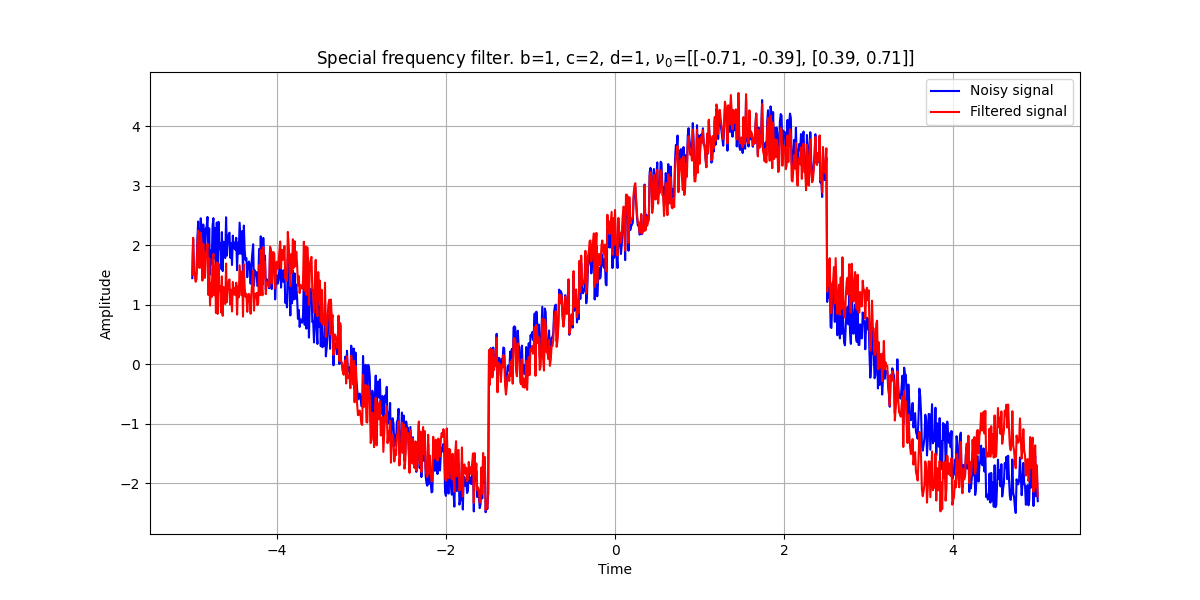
\includegraphics[scale=0.48]{1_u_flt_u_nospec.png}
        \captionsetup{skip=0pt}
        \caption{График исходного и фильтрованного сигналов (1)}
        \label{fig:fig71}
    \end{figure}
    \begin{figure}[!htb]
        \centering
        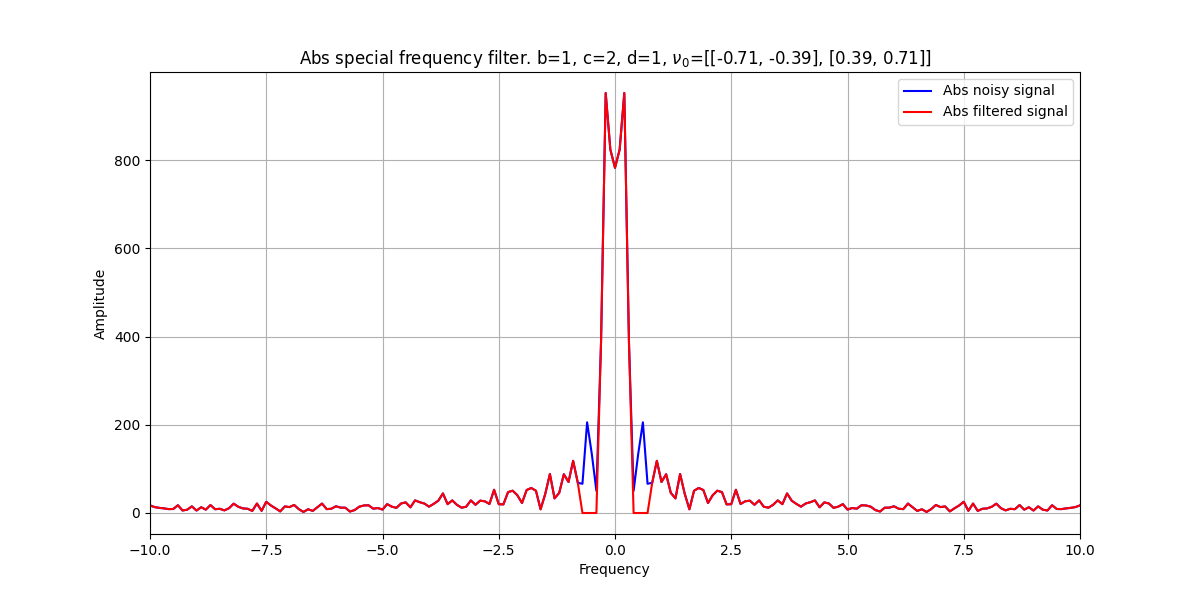
\includegraphics[scale=0.48]{1_abs_u_U_nospec.png}
        \captionsetup{skip=0pt}
        \caption{График модуля Фурье-образа исходного и фильтрованного сигналов (1)}
        \label{fig:fig72}
    \end{figure}
    \begin{figure}[!htb]
        \centering
        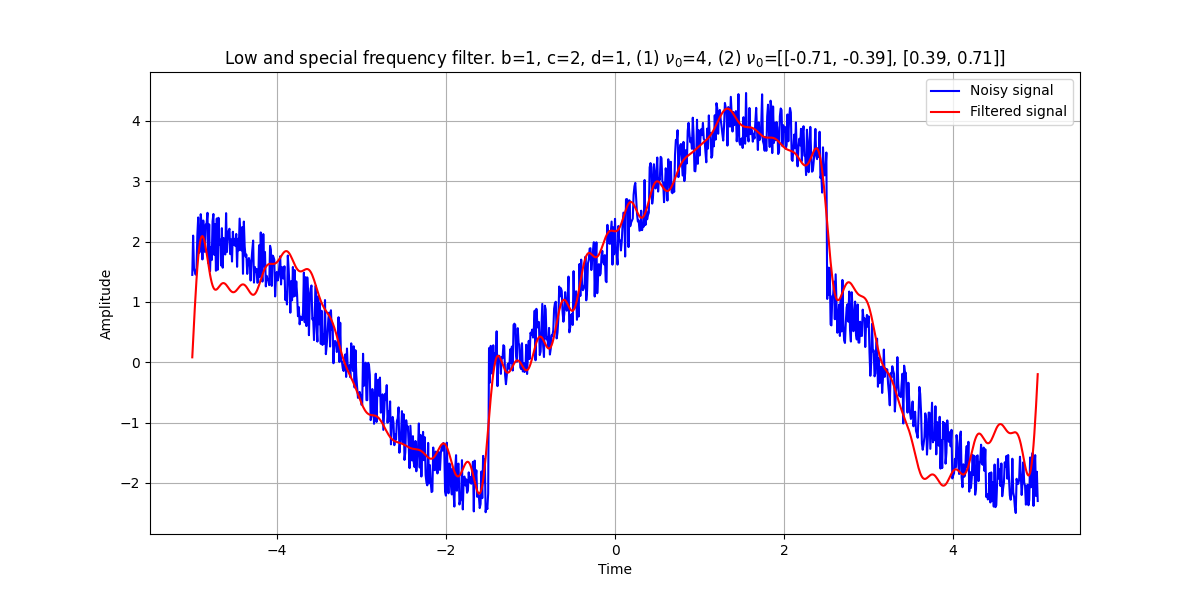
\includegraphics[scale=0.48]{1_3_u_flt_u_nospec.png}
        \captionsetup{skip=0pt}
        \caption{График исходного и фильтрованного сигналов (1)}
        \label{fig:fig77}
    \end{figure}
    \begin{figure}[!htb]
        \centering
        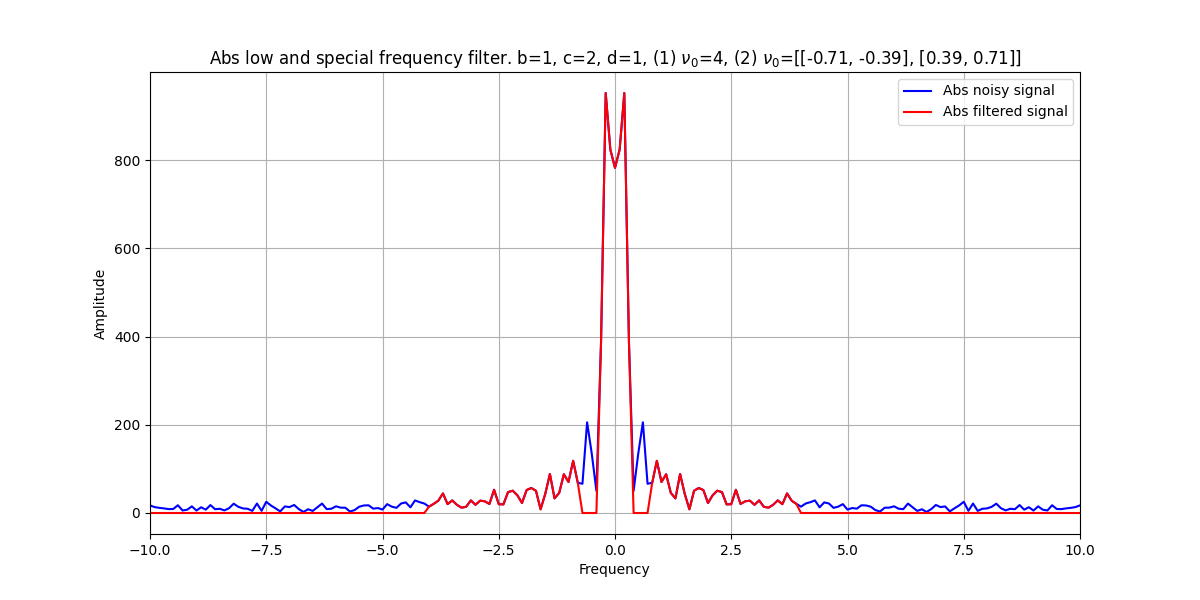
\includegraphics[scale=0.48]{1_3_abs_u_U_nospec.png}
        \captionsetup{skip=0pt}
        \caption{График модуля Фурье-образа исходного и фильтрованного сигналов (1)}
        \label{fig:fig78}
    \end{figure}
    \begin{figure}[!htb]
        \centering
        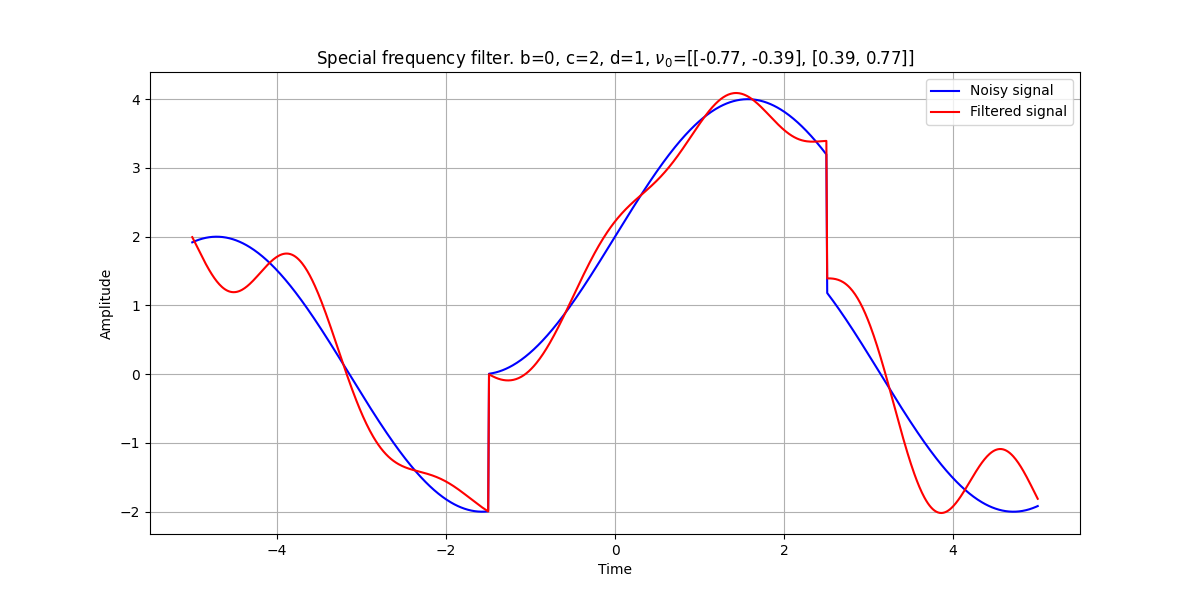
\includegraphics[scale=0.48]{2_u_flt_u_nospec.png}
        \captionsetup{skip=0pt}
        \caption{График исходного и фильтрованного сигналов (2)}
        \label{fig:fig81}
    \end{figure}
    \begin{figure}[!htb]
        \centering
        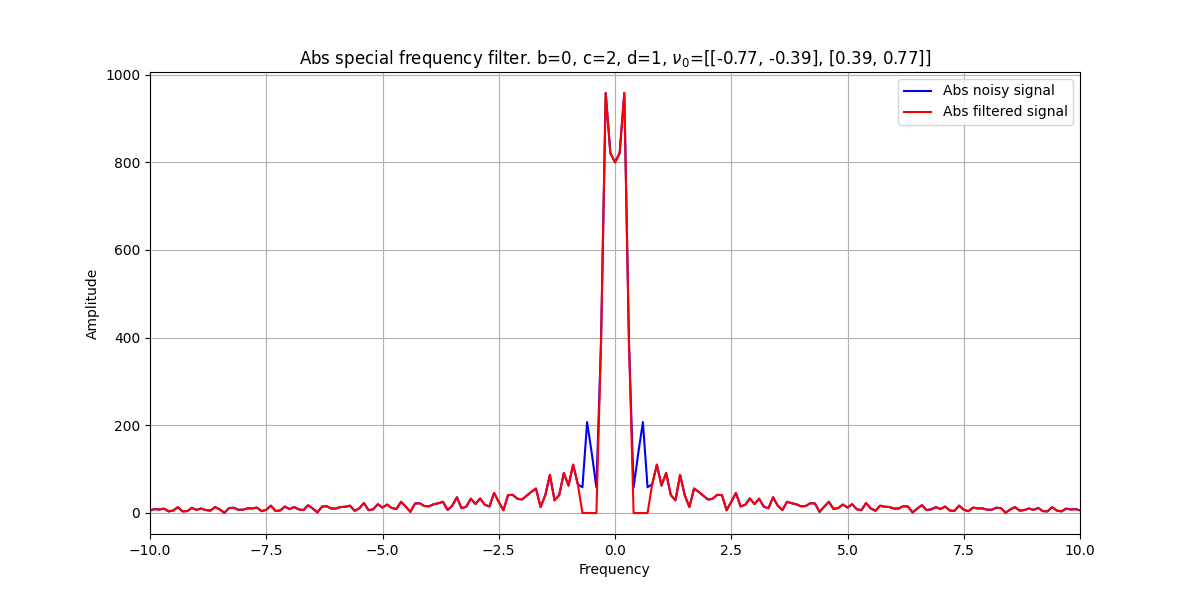
\includegraphics[scale=0.48]{2_abs_u_U_nospec.png}
        \captionsetup{skip=0pt}
        \caption{График модуля Фурье-образа исходного и фильтрованного сигналов (2)}
        \label{fig:fig82}
    \end{figure}
    \begin{figure}[!htb]
        \centering
        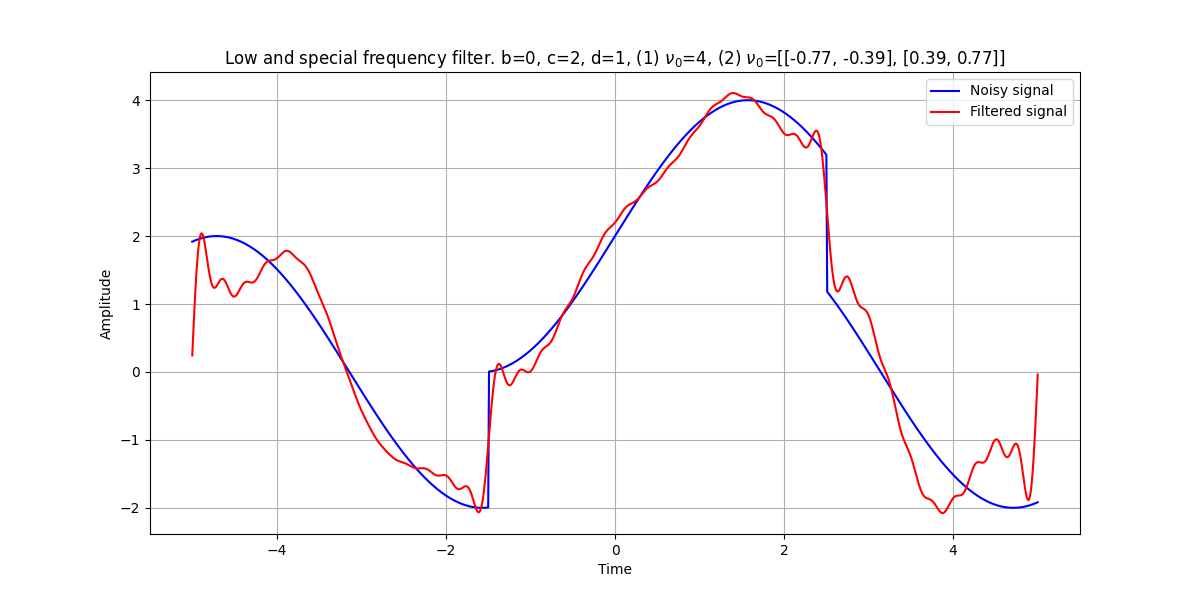
\includegraphics[scale=0.48]{2_3_u_flt_u_nospec.png}
        \captionsetup{skip=0pt}
        \caption{График исходного и фильтрованного сигналов (2)}
        \label{fig:fig87}
    \end{figure}
    \begin{figure}[!htb]
        \centering
        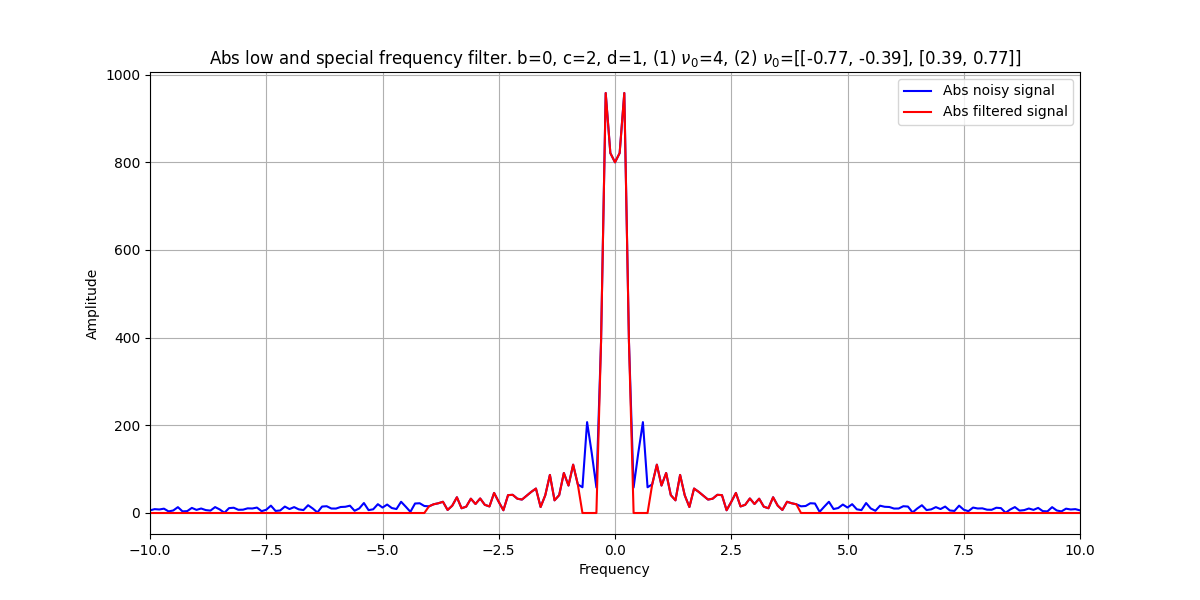
\includegraphics[scale=0.48]{2_3_abs_u_U_nospec.png}
        \captionsetup{skip=0pt}
        \caption{График модуля Фурье-образа исходного и фильтрованного сигналов (2)}
        \label{fig:fig88}
    \end{figure}
    \begin{figure}[!htb]
        \centering
        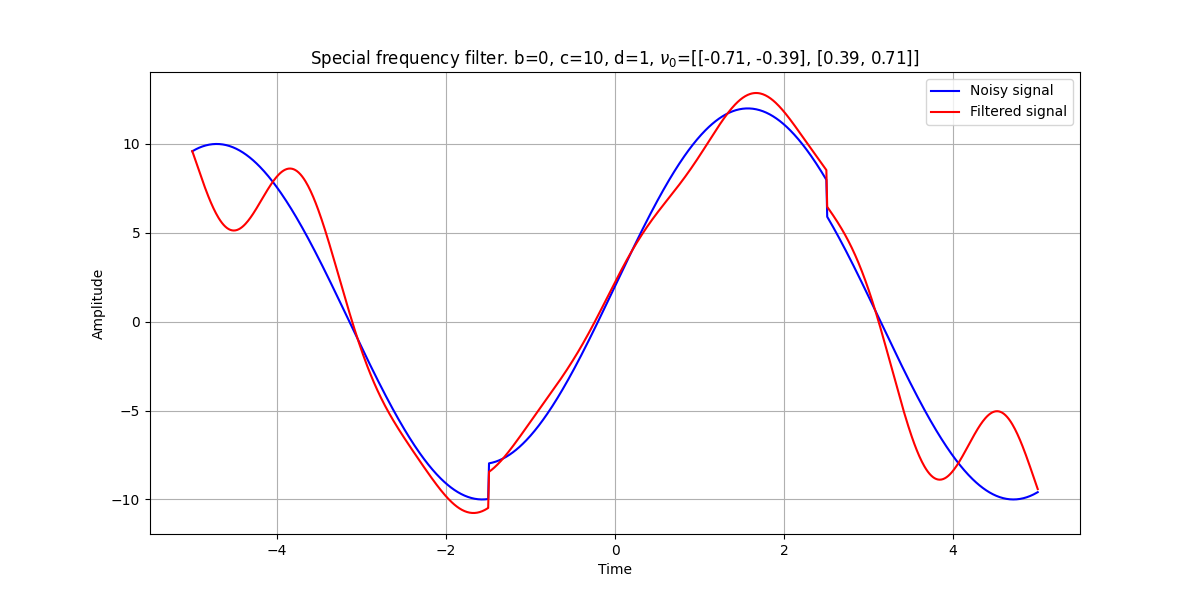
\includegraphics[scale=0.48]{3_u_flt_u_nospec.png}
        \captionsetup{skip=0pt}
        \caption{График исходного и фильтрованного сигналов (3)}
        \label{fig:fig91}
    \end{figure}
    \begin{figure}[!htb]
        \centering
        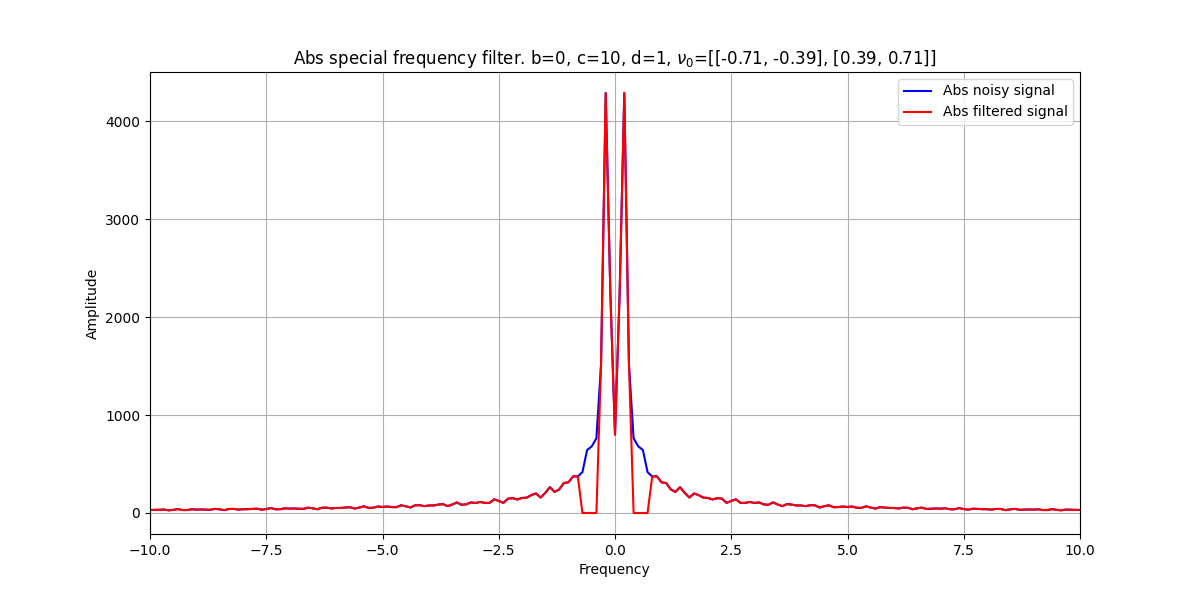
\includegraphics[scale=0.48]{3_abs_u_U_nospec.png}
        \captionsetup{skip=0pt}
        \caption{График модуля Фурье-образа исходного и фильтрованного сигналов (3)}
        \label{fig:fig92}
    \end{figure}
    \begin{figure}[!htb]
        \centering
        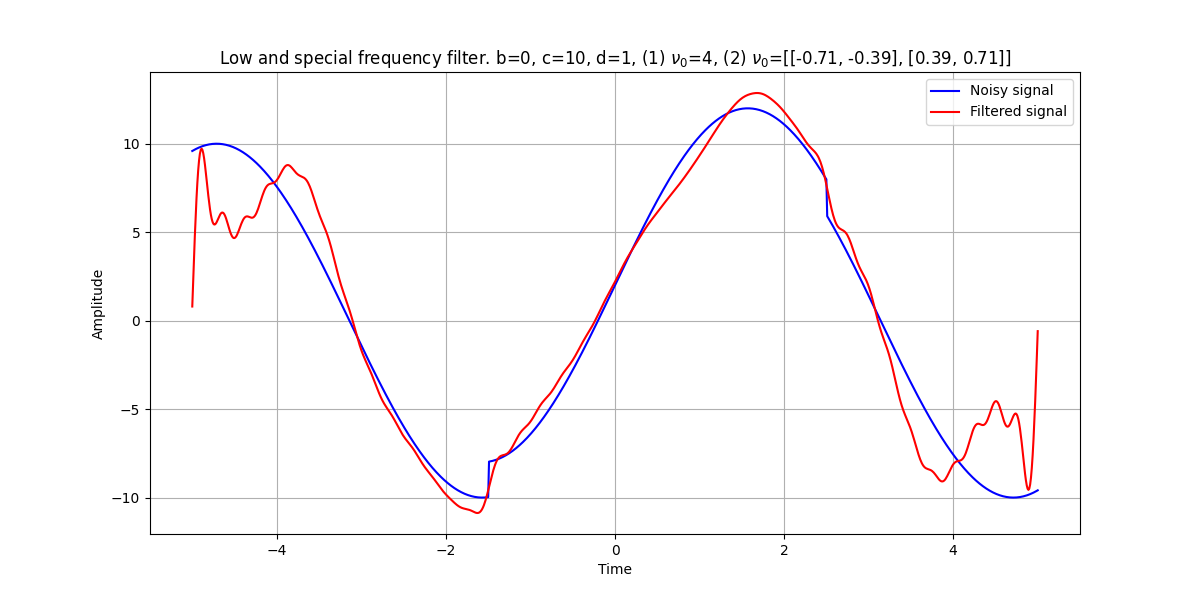
\includegraphics[scale=0.48]{3_3_u_flt_u_nospec.png}
        \captionsetup{skip=0pt}
        \caption{График исходного и фильтрованного сигналов (3)}
        \label{fig:fig97}
    \end{figure}
    \begin{figure}[!htb]
        \centering
        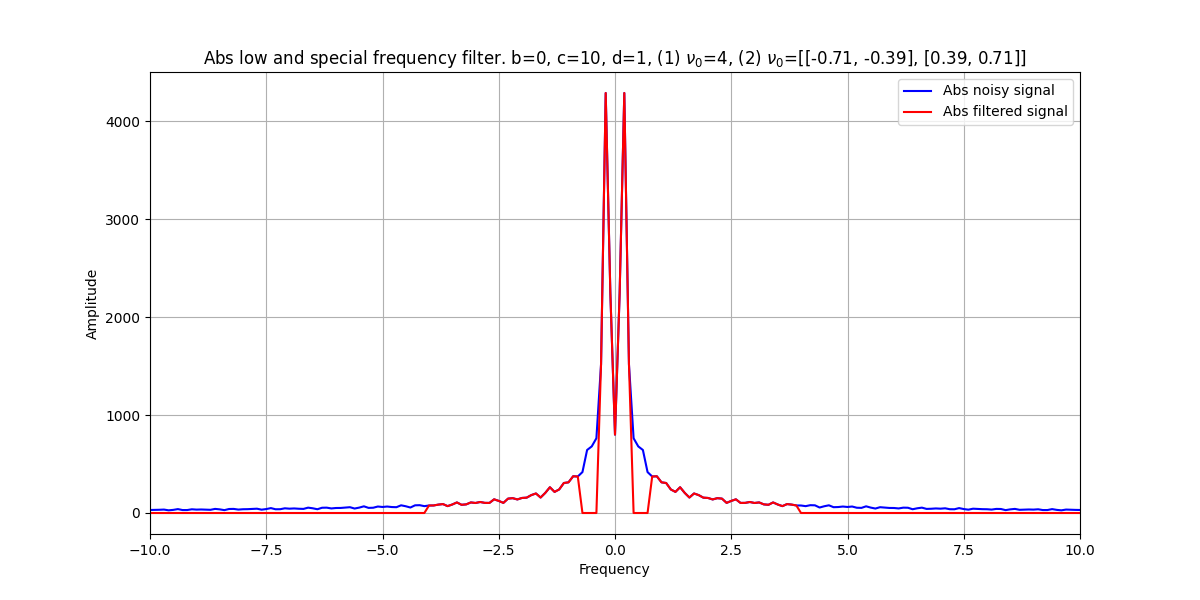
\includegraphics[scale=0.48]{3_3_abs_u_U_nospec.png}
        \captionsetup{skip=0pt}
        \caption{График модуля Фурье-образа исходного и фильтрованного сигналов (3)}
        \label{fig:fig98}
    \end{figure}
    \begin{figure}[!htb]
        \centering
        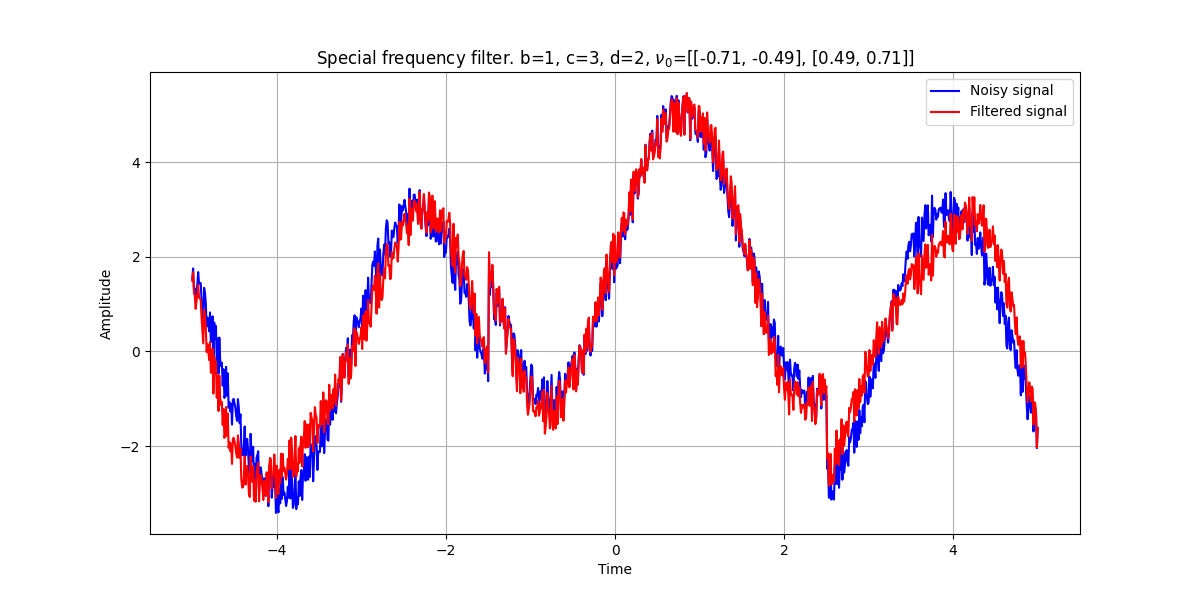
\includegraphics[scale=0.48]{4_u_flt_u_nospec.png}
        \captionsetup{skip=0pt}
        \caption{График исходного и фильтрованного сигналов (4)}
        \label{fig:fig101}
    \end{figure}
    \begin{figure}[!htb]
        \centering
        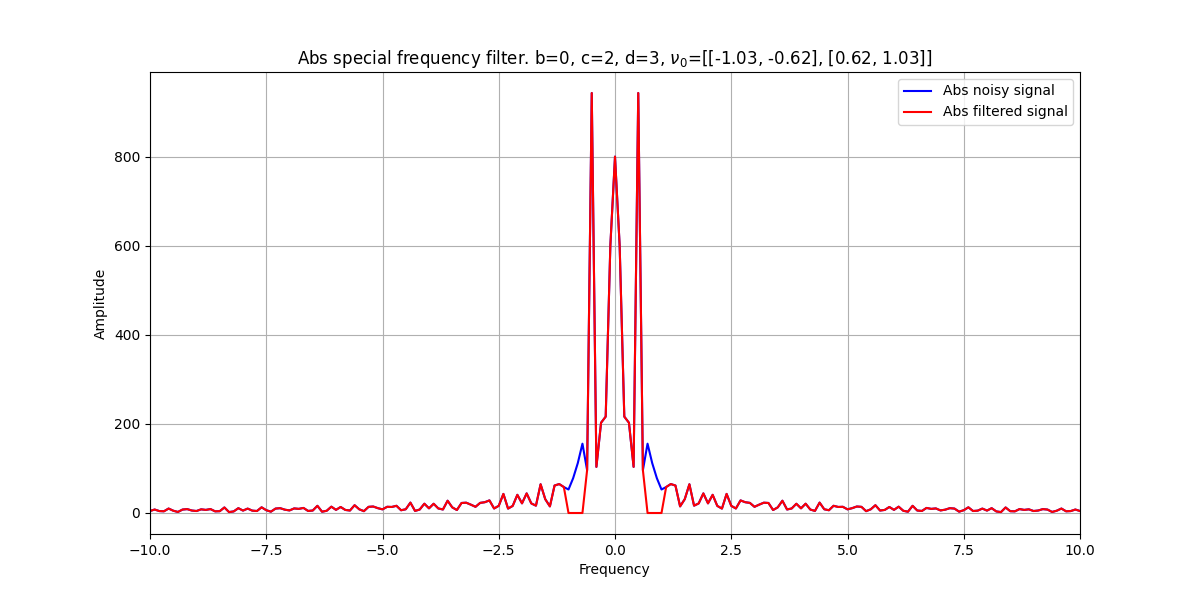
\includegraphics[scale=0.48]{4_abs_u_U_nospec.png}
        \captionsetup{skip=0pt}
        \caption{График модуля Фурье-образа исходного и фильтрованного сигналов (4)}
        \label{fig:fig102}
    \end{figure}
    \begin{figure}[!htb]
        \centering
        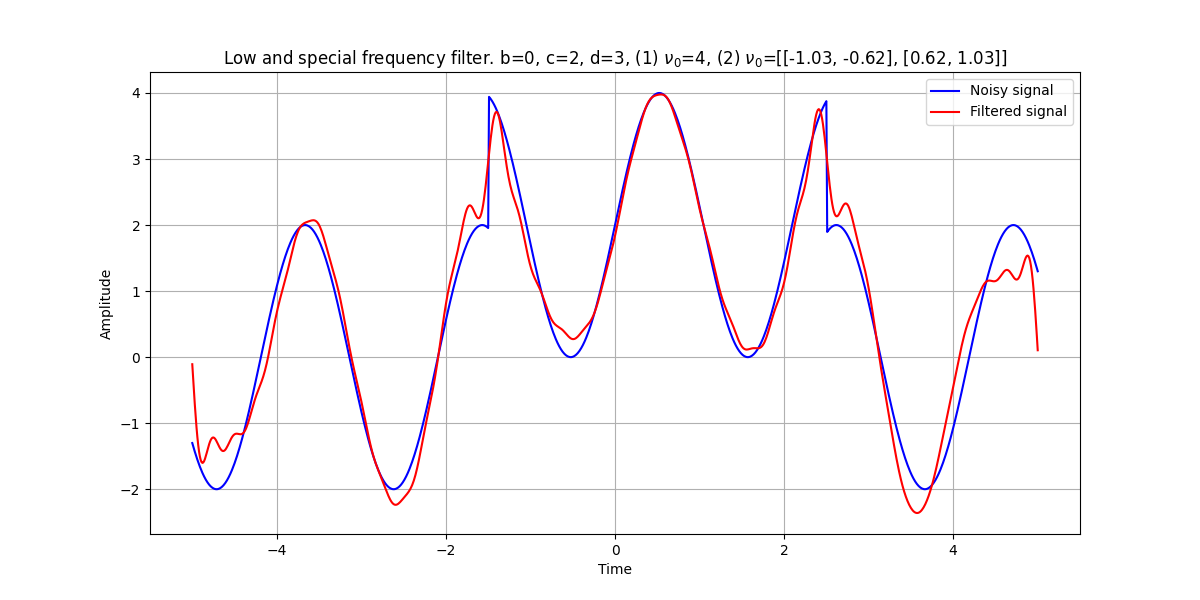
\includegraphics[scale=0.48]{4_3_u_flt_u_nospec.png}
        \captionsetup{skip=0pt}
        \caption{График исходного и фильтрованного сигналов (4)}
        \label{fig:fig107}
    \end{figure}
    \begin{figure}[!htb]
        \centering
        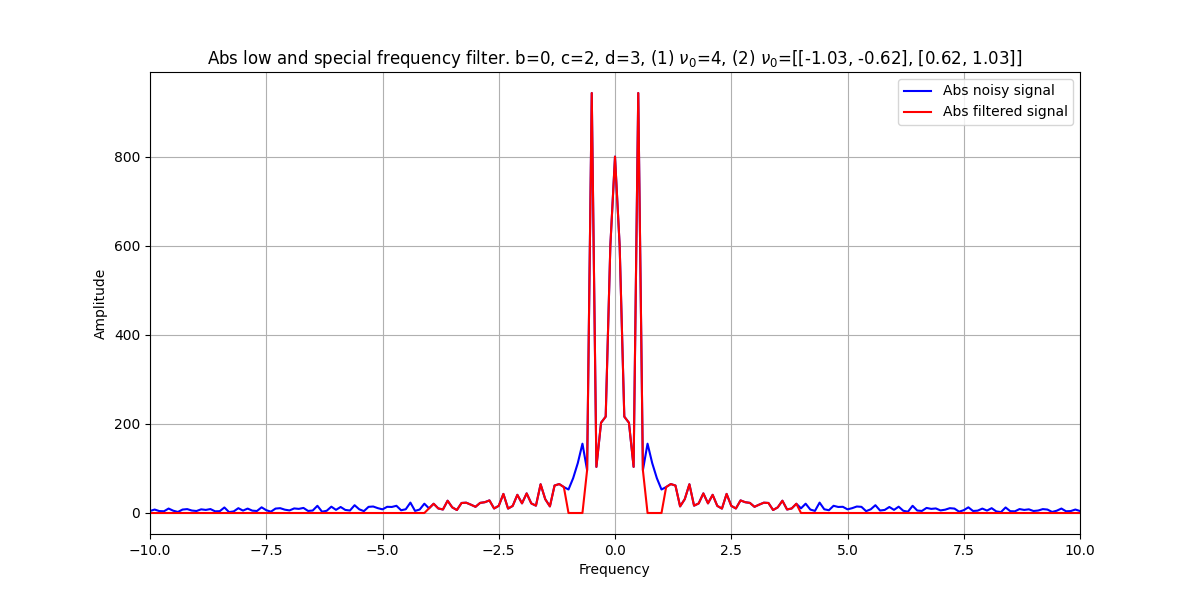
\includegraphics[scale=0.48]{4_3_abs_u_U_nospec.png}
        \captionsetup{skip=0pt}
        \caption{График модуля Фурье-образа исходного и фильтрованного сигналов (4)}
        \label{fig:fig108}
    \end{figure}
    \begin{figure}[!htb]
        \centering
        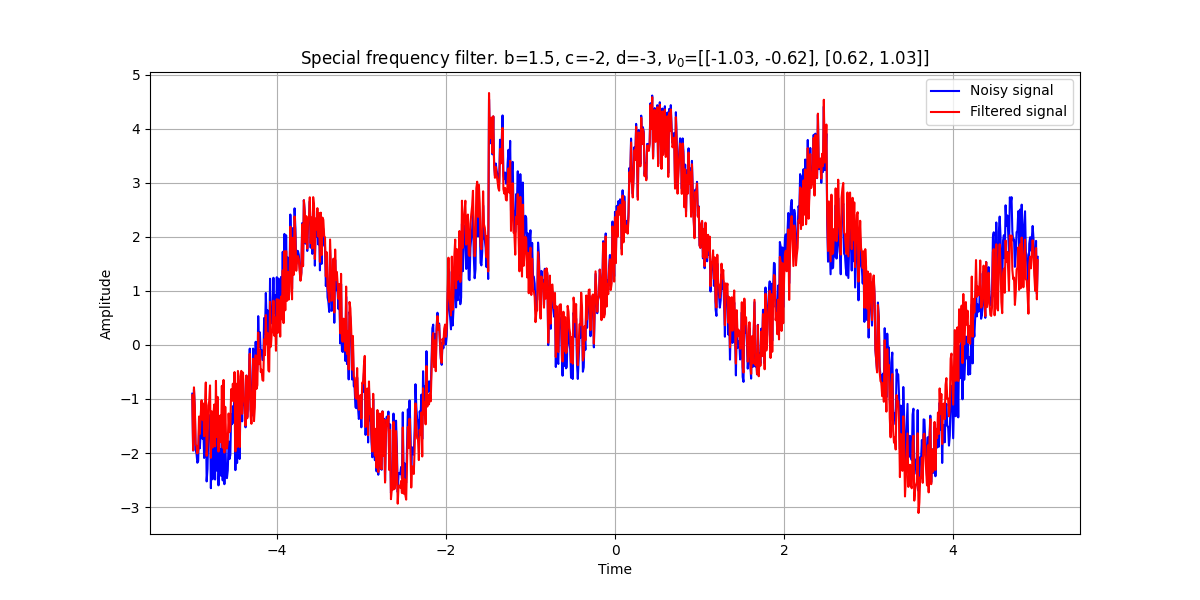
\includegraphics[scale=0.48]{5_u_flt_u_nospec.png}
        \captionsetup{skip=0pt}
        \caption{График исходного и фильтрованного сигналов (5)}
        \label{fig:fig01}
    \end{figure}
    \begin{figure}[!htb]
        \centering
        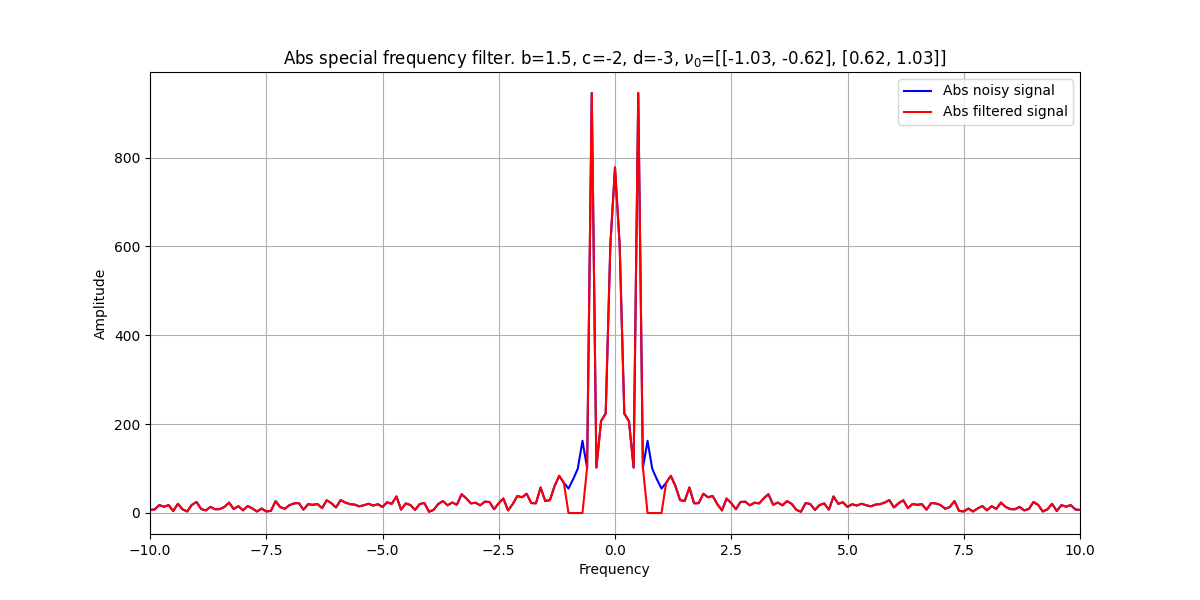
\includegraphics[scale=0.48]{5_abs_u_U_nospec.png}
        \captionsetup{skip=0pt}
        \caption{График модуля Фурье-образа исходного и фильтрованного сигналов (5)}
        \label{fig:fig02}
    \end{figure}
    \begin{figure}[H]
        \centering
        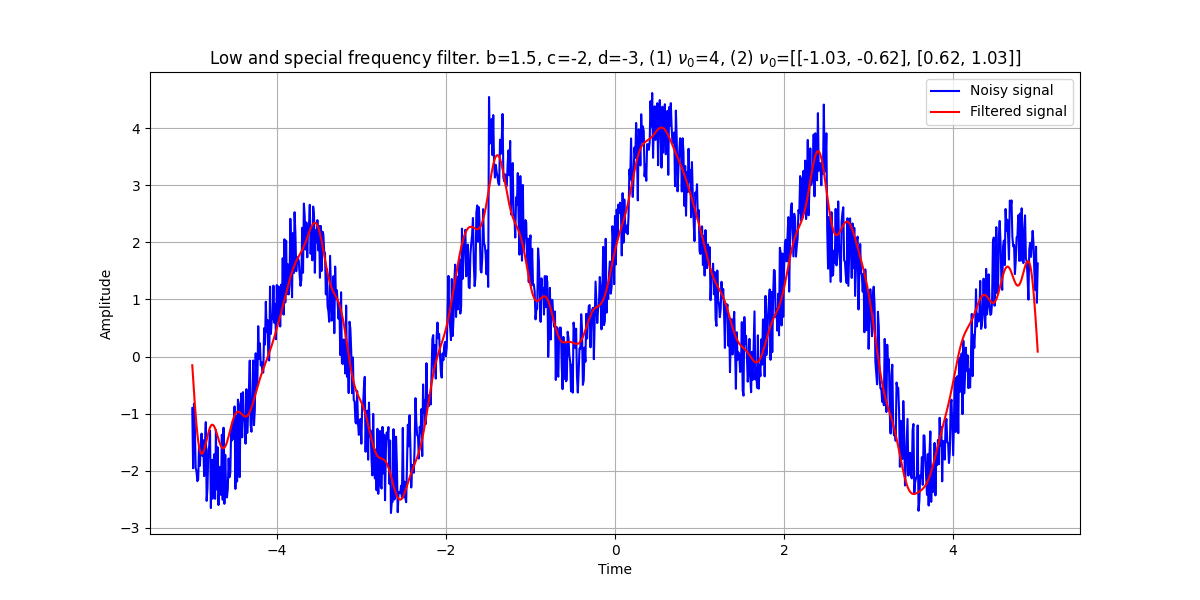
\includegraphics[scale=0.48]{5_3_u_flt_u_nospec.png}
        \captionsetup{skip=0pt}
        \caption{График исходного и фильтрованного сигналов (5)}
        \label{fig:fig07}
    \end{figure}
    \begin{figure}[!htb]
        \centering
        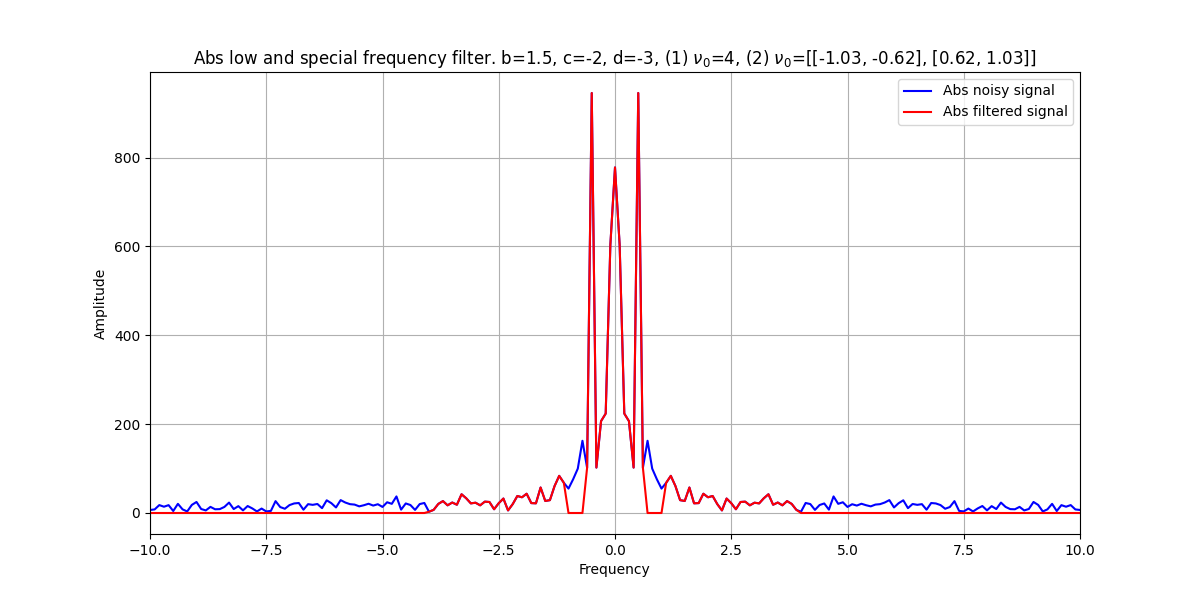
\includegraphics[scale=0.48]{5_3_abs_u_U_nospec.png}
        \captionsetup{skip=0pt}
        \caption{График модуля Фурье-образа исходного и фильтрованного сигналов (5)}
        \label{fig:fig08}
    \end{figure}
    \begin{figure}[!htb]
        \centering
        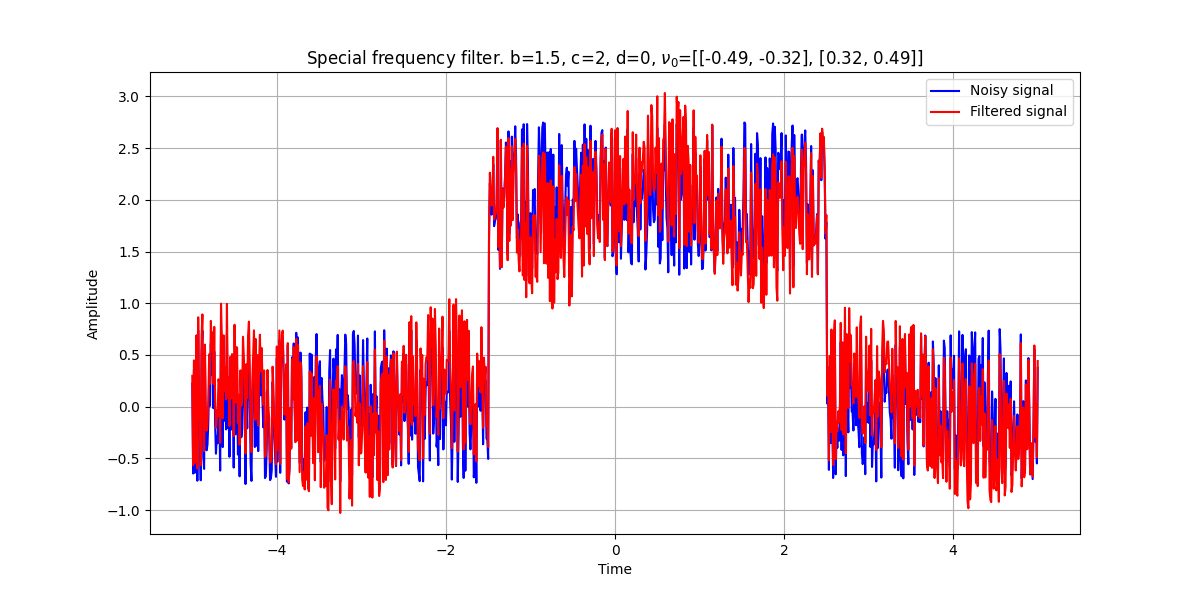
\includegraphics[scale=0.48]{6_u_flt_u_nospec.png}
        \captionsetup{skip=0pt}
        \caption{График исходного и фильтрованного сигналов (6)}
        \label{fig:mlll}
    \end{figure}
    \begin{figure}[!htb]
        \centering
        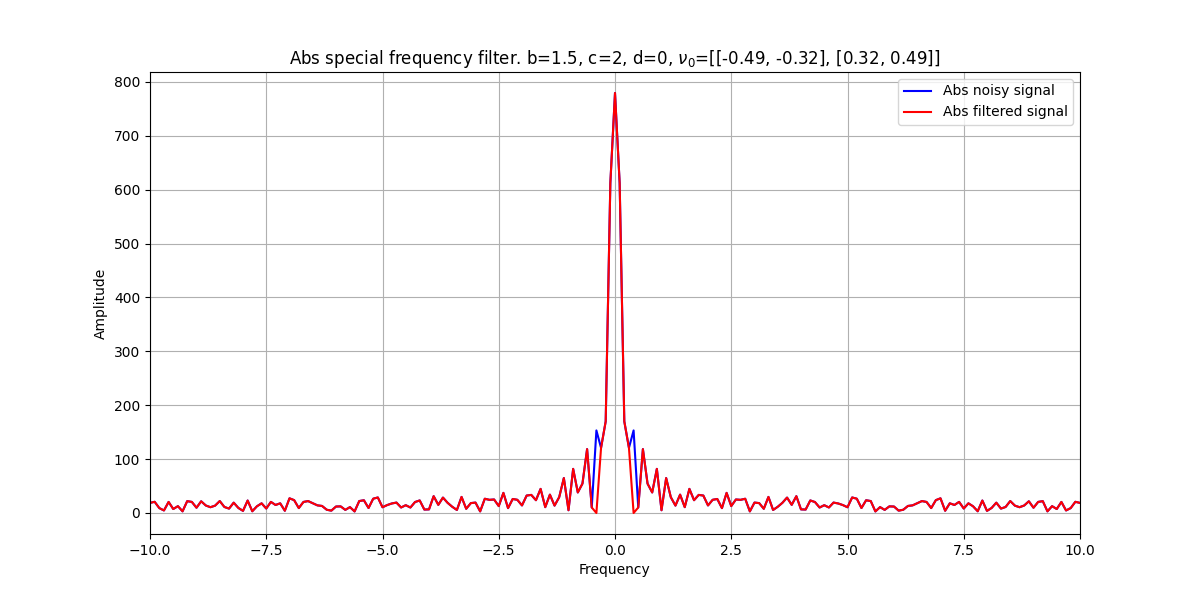
\includegraphics[scale=0.48]{6_abs_u_U_nospec.png}
        \captionsetup{skip=0pt}
        \caption{График модуля Фурье-образа исходного и фильтрованного сигналов (6)}
        \label{fig:dchjdhc}
    \end{figure}
    \begin{figure}[!htb]
        \centering
        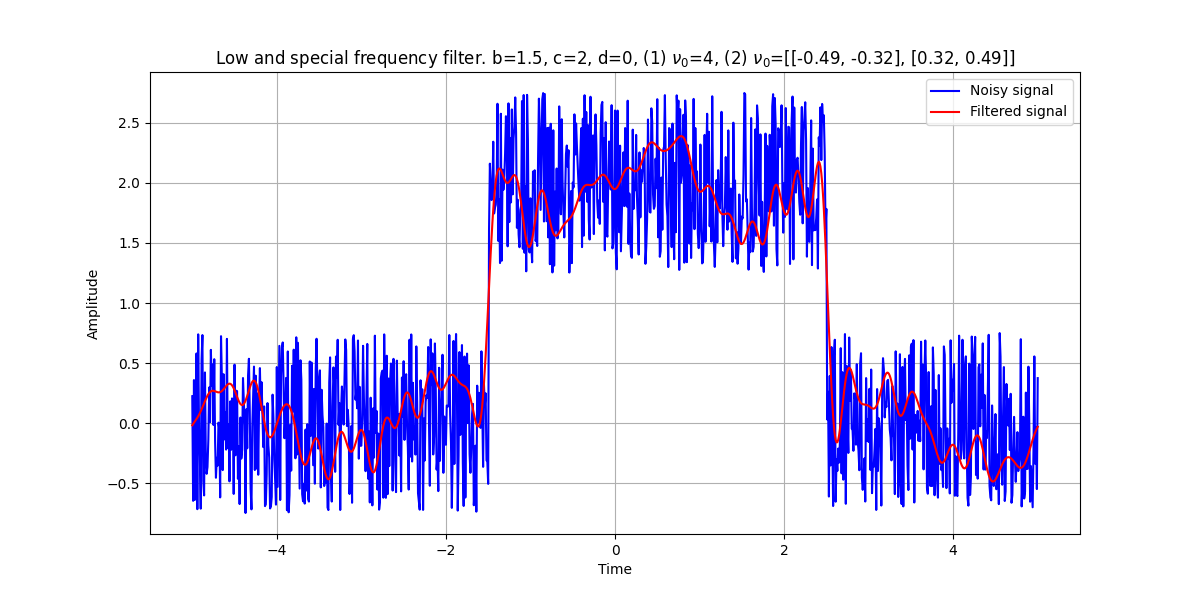
\includegraphics[scale=0.48]{6_3_u_flt_u_nospec.png}
        \captionsetup{skip=0pt}
        \caption{График исходного и фильтрованного сигналов (6)}
        \label{fig:sdjfsdfj}
    \end{figure}
    \begin{figure}[!htb]
        \centering
        \includegraphics[scale=0.48]{6_3_abs_u_U_nospec.png}
        \captionsetup{skip=0pt}
        \caption{График модуля Фурье-образа исходного и фильтрованного сигналов (6)}
        \label{fig:oirjghofgj}
    \end{figure}
    \begin{figure}[!htb]
        \centering
        \includegraphics[scale=0.48]{7_u_flt_u_nospec.png}
        \captionsetup{skip=0pt}
        \caption{График исходного и фильтрованного сигналов (7)}
        \label{fig:dklfksdjfo}
    \end{figure}
    \begin{figure}[H]
        \centering
        \includegraphics[scale=0.48]{7_abs_u_U_nospec.png}
        \captionsetup{skip=0pt}
        \caption{График модуля Фурье-образа исходного и фильтрованного сигналов (7)}
        \label{fig:dfsjusdf}
    \end{figure}
    \begin{figure}[!htb]
        \centering
        \includegraphics[scale=0.48]{7_3_u_flt_u_nospec.png}
        \captionsetup{skip=0pt}
        \caption{График исходного и фильтрованного сигналов (7)}
        \label{fig:fsdjflsfl}
    \end{figure}
    \begin{figure}[H]
        \centering
        \includegraphics[scale=0.48]{7_3_abs_u_U_nospec.png}
        \captionsetup{skip=0pt}
        \caption{График модуля Фурье-образа исходного и фильтрованного сигналов (7)}
        \label{fig:f939}
    \end{figure}
    \begin{figure}[H]
        \centering
        \includegraphics[scale=0.48]{8_u_flt_u_nospec.png}
        \captionsetup{skip=0pt}
        \caption{График исходного и фильтрованного сигналов (8)}
        \label{fig:vbvbv}
    \end{figure}
    \begin{figure}[!htb]
        \centering
        \includegraphics[scale=0.48]{8_abs_u_U_nospec.png}
        \captionsetup{skip=0pt}
        \caption{График модуля Фурье-образа исходного и фильтрованного сигналов (8)}
        \label{fig:wewew}
    \end{figure}
    \begin{figure}[H]
        \centering
        \includegraphics[scale=0.48]{8_3_u_flt_u_nospec.png}
        \captionsetup{skip=0pt}
        \caption{График исходного и фильтрованного сигналов (8)}
        \label{fig:snf}
    \end{figure}
    \begin{figure}[!htb]
        \centering
        \includegraphics[scale=0.48]{8_3_abs_u_U_nospec.png}
        \captionsetup{skip=0pt}
        \caption{График модуля Фурье-образа исходного и фильтрованного сигналов (8)}
        \label{fig:wkljkf}
    \end{figure}


    \subsection{Убираем низкие частоты. Фильтр верхних частот.}
    Рассмотрим графики, где в некоторой окресности точки $\nu=0$ обнулим все значения частот Фурье-образа.
    Такое поведение соответствует фильтру \textit{верхних} частот, так как он пропускает все частоты выше частоты среза.
    Окресность будет настраиваться выбором диапазона частот $[-\nu_0,\nu_0]$. Для лучшей показательности выбраны как маленькие
    окресности около нуля, так и большие. Также рассмотрим поведение фильтрации при различных параметрах $b,\,c,\,d$.


    Далее будут приведены рисунки полученных графиков. На каждом графике подписаны выбранные значения $b,\,c,\,d,\,\nu_0$. 
    Синим цветом обозначается оригинальный сигнал, красным фильтрованный.


    По полученным графикам можно сделать вывод -- фильтр верхних частот в данном случае отрезает значимую часть сигнала,
    содержащуюся в нижних частотах, и оставляет только белый и/или гармонический шум, находящийся преимущественно на высоких частотах.


    \begin{figure}[!htb]
        \centering
        \includegraphics[scale=0.48]{1_u_flt_u_nolow.png}
        \captionsetup{skip=0pt}
        \caption{График исходного и фильтрованного сигналов (1)}
        \label{fig:fig27}
    \end{figure}
    \begin{figure}[!htb]
        \centering
        \includegraphics[scale=0.48]{1_abs_u_U_nolow.png}
        \captionsetup{skip=0pt}
        \caption{График модуля Фурье-образа исходного и фильтрованного сигналов (1)}
        \label{fig:fig28}
    \end{figure}
    \begin{figure}[!htb]
        \centering
        \includegraphics[scale=0.48]{2_u_flt_u_nolow.png}
        \captionsetup{skip=0pt}
        \caption{График исходного и фильтрованного сигналов (2)}
        \label{fig:fig29}
    \end{figure}
    \begin{figure}[H]
        \centering
        \includegraphics[scale=0.48]{2_abs_u_U_nolow.png}
        \captionsetup{skip=0pt}
        \caption{График модуля Фурье-образа исходного и фильтрованного сигналов (2)}
        \label{fig:fig30}
    \end{figure}
    \begin{figure}[!htb]
        \centering
        \includegraphics[scale=0.48]{3_u_flt_u_nolow.png}
        \captionsetup{skip=0pt}
        \caption{График исходного и фильтрованного сигналов (3)}
        \label{fig:fig31}
    \end{figure}
    \begin{figure}[!htb]
        \centering
        \includegraphics[scale=0.48]{3_abs_u_U_nolow.png}
        \captionsetup{skip=0pt}
        \caption{График модуля Фурье-образа исходного и фильтрованного сигналов (3)}
        \label{fig:fig32}
    \end{figure}
    \begin{figure}[!htb]
        \centering
        \includegraphics[scale=0.48]{4_u_flt_u_nolow.png}
        \captionsetup{skip=0pt}
        \caption{График исходного и фильтрованного сигналов (4)}
        \label{fig:fig33}
    \end{figure}
    \begin{figure}[!htb]
        \centering
        \includegraphics[scale=0.48]{4_abs_u_U_nolow.png}
        \captionsetup{skip=0pt}
        \caption{График модуля Фурье-образа исходного и фильтрованного сигналов (4)}
        \label{fig:fig34}
    \end{figure}
    \begin{figure}[!htb]
        \centering
        \includegraphics[scale=0.48]{5_u_flt_u_nolow.png}
        \captionsetup{skip=0pt}
        \caption{График исходного и фильтрованного сигналов (5)}
        \label{fig:fig35}
    \end{figure}
    \begin{figure}[!htb]
        \centering
        \includegraphics[scale=0.48]{5_abs_u_U_nolow.png}
        \captionsetup{skip=0pt}
        \caption{График модуля Фурье-образа исходного и фильтрованного сигналов (5)}
        \label{fig:fig36}
    \end{figure}
    \begin{figure}[!htb]
        \centering
        \includegraphics[scale=0.48]{6_u_flt_u_nolow.png}
        \captionsetup{skip=0pt}
        \caption{График исходного и фильтрованного сигналов (6)}
        \label{fig:fig37}
    \end{figure}
    \begin{figure}[!htb]
        \centering
        \includegraphics[scale=0.48]{6_abs_u_U_nolow.png}
        \captionsetup{skip=0pt}
        \caption{График модуля Фурье-образа исходного и фильтрованного сигналов (6)}
        \label{fig:fig38}
    \end{figure}
    \begin{figure}[!htb]
        \centering
        \includegraphics[scale=0.48]{7_u_flt_u_nolow.png}
        \captionsetup{skip=0pt}
        \caption{График исходного и фильтрованного сигналов (7)}
        \label{fig:fig39}
    \end{figure}
    \begin{figure}[!htb]
        \centering
        \includegraphics[scale=0.48]{7_abs_u_U_nolow.png}
        \captionsetup{skip=0pt}
        \caption{График модуля Фурье-образа исходного и фильтрованного сигналов (7)}
        \label{fig:fig40}
    \end{figure}
    \begin{figure}[!htb]
        \centering
        \includegraphics[scale=0.48]{8_u_flt_u_nolow.png}
        \captionsetup{skip=0pt}
        \caption{График исходного и фильтрованного сигналов (8)}
        \label{fig:fig41}
    \end{figure}
    \begin{figure}[!htb]
        \centering
        \includegraphics[scale=0.48]{8_abs_u_U_nolow.png}
        \captionsetup{skip=0pt}
        \caption{График модуля Фурье-образа исходного и фильтрованного сигналов (8)}
        \label{fig:fig42}
    \end{figure}
    \begin{figure}[!htb]
        \centering
        \includegraphics[scale=0.48]{9_u_flt_u_nolow.png}
        \captionsetup{skip=0pt}
        \caption{График исходного и фильтрованного сигналов (9)}
        \label{fig:fig43}
    \end{figure}
    \begin{figure}[!htb]
        \centering
        \includegraphics[scale=0.48]{9_abs_u_U_nolow.png}
        \captionsetup{skip=0pt}
        \caption{График модуля Фурье-образа исходного и фильтрованного сигналов (9)}
        \label{fig:fig44}
    \end{figure}
    \begin{figure}[!htb]
        \centering
        \includegraphics[scale=0.48]{10_u_flt_u_nolow.png}
        \captionsetup{skip=0pt}
        \caption{График исходного и фильтрованного сигналов (10)}
        \label{fig:fig45}
    \end{figure}
    \begin{figure}[!htb]
        \centering
        \includegraphics[scale=0.48]{10_abs_u_U_nolow.png}
        \captionsetup{skip=0pt}
        \caption{График модуля Фурье-образа исходного и фильтрованного сигналов (10)}
        \label{fig:fig46}
    \end{figure}
    \begin{figure}[!htb]
        \centering
        \includegraphics[scale=0.48]{11_u_flt_u_nolow.png}
        \captionsetup{skip=0pt}
        \caption{График исходного и фильтрованного сигналов (11)}
        \label{fig:fig47}
    \end{figure}
    \begin{figure}[!htb]
        \centering
        \includegraphics[scale=0.48]{11_abs_u_U_nolow.png}
        \captionsetup{skip=0pt}
        \caption{График модуля Фурье-образа исходного и фильтрованного сигналов (11)}
        \label{fig:fig48}
    \end{figure}
    \begin{figure}[!htb]
        \centering
        \includegraphics[scale=0.48]{12_u_flt_u_nolow.png}
        \captionsetup{skip=0pt}
        \caption{График исходного и фильтрованного сигналов (12)}
        \label{fig:fig49}
    \end{figure}
    \begin{figure}[!htb]
        \centering
        \includegraphics[scale=0.48]{12_abs_u_U_nolow.png}
        \captionsetup{skip=0pt}
        \caption{График модуля Фурье-образа исходного и фильтрованного сигналов (12)}
        \label{fig:fig50}
    \end{figure}
    \begin{figure}[!htb]
        \centering
        \includegraphics[scale=0.48]{13_u_flt_u_nolow.png}
        \captionsetup{skip=0pt}
        \caption{График исходного и фильтрованного сигналов (13)}
        \label{fig:fig51}
    \end{figure}
    \begin{figure}[!htb]
        \centering
        \includegraphics[scale=0.48]{13_abs_u_U_nolow.png}
        \captionsetup{skip=0pt}
        \caption{График модуля Фурье-образа исходного и фильтрованного сигналов (13)}
        \label{fig:fig52}
    \end{figure}
    \begin{figure}[!htb]
        \centering
        \includegraphics[scale=0.48]{14_u_flt_u_nolow.png}
        \captionsetup{skip=0pt}
        \caption{График исходного и фильтрованного сигналов (14)}
        \label{fig:fig53}
    \end{figure}
    \begin{figure}[!htb]
        \centering
        \includegraphics[scale=0.48]{14_abs_u_U_nolow.png}
        \captionsetup{skip=0pt}
        \caption{График модуля Фурье-образа исходного и фильтрованного сигналов (14)}
        \label{fig:fig54}
    \end{figure}
    \begin{figure}[!htb]
        \centering
        \includegraphics[scale=0.48]{15_u_flt_u_nolow.png}
        \captionsetup{skip=0pt}
        \caption{График исходного и фильтрованного сигналов (15)}
        \label{fig:fig55}
    \end{figure}
    \begin{figure}[!htb]
        \centering
        \includegraphics[scale=0.48]{15_abs_u_U_nolow.png}
        \captionsetup{skip=0pt}
        \caption{График модуля Фурье-образа исходного и фильтрованного сигналов (15)}
        \label{fig:fig56}
    \end{figure}
    \begin{figure}[!htb]
        \centering
        \includegraphics[scale=0.48]{16_u_flt_u_nolow.png}
        \captionsetup{skip=0pt}
        \caption{График исходного и фильтрованного сигналов (16)}
        \label{fig:fig57}
    \end{figure}
    \begin{figure}[!htb]
        \centering
        \includegraphics[scale=0.48]{16_abs_u_U_nolow.png}
        \captionsetup{skip=0pt}
        \caption{График модуля Фурье-образа исходного и фильтрованного сигналов (16)}
        \label{fig:fig58}
    \end{figure}
    \begin{figure}[!htb]
        \centering
        \includegraphics[scale=0.48]{17_u_flt_u_nolow.png}
        \captionsetup{skip=0pt}
        \caption{График исходного и фильтрованного сигналов (17)}
        \label{fig:fig59}
    \end{figure}
    \begin{figure}[!htb]
        \centering
        \includegraphics[scale=0.48]{17_abs_u_U_nolow.png}
        \captionsetup{skip=0pt}
        \caption{График модуля Фурье-образа исходного и фильтрованного сигналов (17)}
        \label{fig:fig60}
    \end{figure}
    \begin{figure}[!htb]
        \centering
        \includegraphics[scale=0.48]{18_u_flt_u_nolow.png}
        \captionsetup{skip=0pt}
        \caption{График исходного и фильтрованного сигналов (18)}
        \label{fig:fig61}
    \end{figure}
    \begin{figure}[!htb]
        \centering
        \includegraphics[scale=0.48]{18_abs_u_U_nolow.png}
        \captionsetup{skip=0pt}
        \caption{График модуля Фурье-образа исходного и фильтрованного сигналов (18)}
        \label{fig:fig62}
    \end{figure}
    \begin{figure}[!htb]
        \centering
        \includegraphics[scale=0.48]{19_u_flt_u_nolow.png}
        \captionsetup{skip=0pt}
        \caption{График исходного и фильтрованного сигналов (19)}
        \label{fig:fig63}
    \end{figure}
    \begin{figure}[!htb]
        \centering
        \includegraphics[scale=0.48]{19_abs_u_U_nolow.png}
        \captionsetup{skip=0pt}
        \caption{График модуля Фурье-образа исходного и фильтрованного сигналов (19)}
        \label{fig:fig64}
    \end{figure}
    \begin{figure}[!htb]
        \centering
        \includegraphics[scale=0.48]{20_u_flt_u_nolow.png}
        \captionsetup{skip=0pt}
        \caption{График исходного и фильтрованного сигналов (20)}
        \label{fig:fig65}
    \end{figure}
    \begin{figure}[!htb]
        \centering
        \includegraphics[scale=0.48]{20_abs_u_U_nolow.png}
        \captionsetup{skip=0pt}
        \caption{График модуля Фурье-образа исходного и фильтрованного сигналов (20)}
        \label{fig:fig66}
    \end{figure}
    \begin{figure}[!htb]
        \centering
        \includegraphics[scale=0.48]{21_u_flt_u_nolow.png}
        \captionsetup{skip=0pt}
        \caption{График исходного и фильтрованного сигналов (21)}
        \label{fig:fig67}
    \end{figure}
    \begin{figure}[!htb]
        \centering
        \includegraphics[scale=0.48]{21_abs_u_U_nolow.png}
        \captionsetup{skip=0pt}
        \caption{График модуля Фурье-образа исходного и фильтрованного сигналов (21)}
        \label{fig:fig68}
    \end{figure}
    \begin{figure}[!htb]
        \centering
        \includegraphics[scale=0.48]{22_u_flt_u_nolow.png}
        \captionsetup{skip=0pt}
        \caption{График исходного и фильтрованного сигналов (22)}
        \label{fig:fig_a}
    \end{figure}
    \begin{figure}[!htb]
        \centering
        \includegraphics[scale=0.48]{22_abs_u_U_nolow.png}
        \captionsetup{skip=0pt}
        \caption{График модуля Фурье-образа исходного и фильтрованного сигналов (22)}
        \label{fig:fig_b}
    \end{figure}
    \begin{figure}[!htb]
        \centering
        \includegraphics[scale=0.48]{23_u_flt_u_nolow.png}
        \captionsetup{skip=0pt}
        \caption{График исходного и фильтрованного сигналов (23)}
        \label{fig:fig_c}
    \end{figure}
    \begin{figure}[!htb]
        \centering
        \includegraphics[scale=0.48]{23_abs_u_U_nolow.png}
        \captionsetup{skip=0pt}
        \caption{График модуля Фурье-образа исходного и фильтрованного сигналов (23)}
        \label{fig:fig_d}
    \end{figure}
    \begin{figure}[!htb]
        \centering
        \includegraphics[scale=0.48]{24_u_flt_u_nolow.png}
        \captionsetup{skip=0pt}
        \caption{График исходного и фильтрованного сигналов (24)}
        \label{fig:fig_e}
    \end{figure}
    \begin{figure}[!htb]
        \centering
        \includegraphics[scale=0.48]{24_abs_u_U_nolow.png}
        \captionsetup{skip=0pt}
        \caption{График модуля Фурье-образа исходного и фильтрованного сигналов (24)}
        \label{fig:fig_f}
    \end{figure}
    \begin{figure}[!htb]
        \centering
        \includegraphics[scale=0.48]{25_u_flt_u_nolow.png}
        \captionsetup{skip=0pt}
        \caption{График исходного и фильтрованного сигналов (25)}
        \label{fig:fig_g}
    \end{figure}
    \begin{figure}[!htb]
        \centering
        \includegraphics[scale=0.48]{25_abs_u_U_nolow.png}
        \captionsetup{skip=0pt}
        \caption{График модуля Фурье-образа исходного и фильтрованного сигналов (25)}
        \label{fig:fig_h}
    \end{figure}
    \begin{figure}[!htb]
        \centering
        \includegraphics[scale=0.48]{26_u_flt_u_nolow.png}
        \captionsetup{skip=0pt}
        \caption{График исходного и фильтрованного сигналов (26)}
        \label{fig:fig_323234}
    \end{figure}
    \begin{figure}[!htb]
        \centering
        \includegraphics[scale=0.48]{26_abs_u_U_nolow.png}
        \captionsetup{skip=0pt}
        \caption{График модуля Фурье-образа исходного и фильтрованного сигналов (26)}
        \label{fig:fig_56456}
    \end{figure}


    \section{Задание 2. Фильтрация звука.}
    В данном задании необходимо убрать шумы из записи голоса в файле MUHA.wav так, чтобы остался только голос. 
    При прослушивании записи голос слышно не очень хорошо, так как присутствует громкий гул. Построим графики
    исходного сигнала аудиозаписи и его Фурье-образа. Определим по второму графику, какие частоты могут создавать
    шумы. Так как гул громкий, нам необходимо вырезать частоты из аудиозаписи, имеющие наибольшую амплитуду. Такие частоты мы можем
    наблюдать примерно в диапазоне $[-300,300]$ Гц. Чтобы вырезать эти частоты, потребуется фильтр верхних частот, который
    мы рассматривали в задании 1. После применения фильтра построим сравнительный график исходного и фильтрованного
    сигналов аудиозаписи. Можем наблюдать, насколько чище стал сигнал -- оставшиеся амплитуды являются голосом, который 
    нам нужен. Это легко понять исходя из того, что между каждым возрастанием амплитуд есть интервал с падением амплитуд, 
    где они находится в некоторой окресности нуля -- это паузы в предложении, которое говорит человек на записи. Также построим
    сравнительный график модуля исходного и фильтрованного сигналов аудиозаписи. На нем мы видим, что мы успешно вырезали
    низкие частоты с наибольшей амплитудой, которые соответствовали громкому гулу. Теперь послушаем аудиозапись filtered\_{MUHA}.wav, которая 
    оставлена на этом \href{https://drive.google.com/drive/folders/1AuXIiKRWvXFOtJqV3uqPzC494zZ7vCrd?usp=sharing}{гугл-диске}, 
    и убедимся в том, что все посторонние шумы пропали. На записи голос слышно хорошо, однако остался некоторый звуковой эффект 
    фейзер. Избавиться от него удалось обрезав частоты в диапазоне $[-22050, -1000]$ и $[1000, 22050]$ Гц, то есть применив фильтр нижних частот,
    однако голос сильно потерял в качестве. Прослушать этот вариант можно на том же
    \href{https://drive.google.com/drive/folders/1AuXIiKRWvXFOtJqV3uqPzC494zZ7vCrd?usp=sharing}{гугл-диске},
    файл выложен под названием filtered\_{MUHA}\_{2}.wav.


    Далее представлены рисунки с графиками, о которых говорилось в предыдущем абзаце. Синим цветом обозначен исходный сигнал,
    красным -- фильтрованный. Также представлены графики для фильтрованной аудиозаписи filtered\_{MUHA}\_{2}.wav. Стоит заметить,
    что на рисунке \ref{fig:fig116} видно, как окресность нуля стала меньше по сравнению с рисунком \ref{fig:fig113}, то есть в 
    подобных диапазонах амплитуды частот уменьшились (убрали высокочастотный эффект фейзер, оставив диапазон с низкими частотами, но
    без тех, что создавали громкий гул).


    \begin{figure}[!htb]
        \centering
        \includegraphics[scale=0.48]{noisy_audio.png}
        \captionsetup{skip=0pt}
        \caption{График исходного сигнала аудиозаписи.}
        \label{fig:fig111}
    \end{figure}
    \begin{figure}[!htb]
        \centering
        \includegraphics[scale=0.48]{U_audio.png}
        \captionsetup{skip=0pt}
        \caption{График Фурье-образа исходного сигнала аудиозаписи.}
        \label{fig:fig112}
    \end{figure}
    \begin{figure}[!htb]
        \centering
        \includegraphics[scale=0.48]{u_flt_u_audio.png}
        \captionsetup{skip=0pt}
        \caption{График исходного и фильтрованного сигналов аудиозаписи (1)}
        \label{fig:fig113}
    \end{figure}
    \begin{figure}[!htb]
        \centering
        \includegraphics[scale=0.48]{abs_u_U_audio.png}
        \captionsetup{skip=0pt}
        \caption{График модуля Фурье-образа исходного и фильтрованного сигналов аудиозаписи (1)}
        \label{fig:fig114}
    \end{figure}
    \begin{figure}[!htb]
        \centering
        \includegraphics[scale=0.48]{u_flt_u_audio_v2.png}
        \captionsetup{skip=0pt}
        \caption{График исходного и фильтрованного сигналов аудиозаписи (2)}
        \label{fig:fig115}
    \end{figure}
    \begin{figure}[H]
        \centering
        \includegraphics[scale=0.48]{abs_u_U_audio_v2.png}
        \captionsetup{skip=0pt}
        \caption{График модуля Фурье-образа исходного и фильтрованного сигналов аудиозаписи (2)}
        \label{fig:fig116}
    \end{figure}

    
    \section{Листинги программных реализаций}
    В этой секции будут рассмотрены программные реализации, которые использовались по ходу выполнения лабораторной работы.
    Программы написаны на языке python с подключенными библиотеками numpy и matplotlib.


    Два файла, которые необходимы для задания массива времени и частот, вычисления массива функций $g$, задания
    сигнала $u$, а также подсчета Фурье-образа сигнала $u$. Достаточно передать в функции необходимые параметры и
    далее их результат можно использовать для выполнения фильтрации и построения графиков.


    \begin{lstlisting}[label=l1, caption={Файл help.py. Вспомогательные функции}]
    def get_t(T, dt):
        return np.arange(-T/2, T/2 + dt, dt)   
        
    def get_v(V, dv):
        return np.arange(-V/2, V/2 + dv, dv)
          
    def get_U(u):
        return np.fft.fftshift(np.fft.fft(u))
        
    def g_f(t, t_1, t_2, a):
        if (t_1 <= t <= t_2):
            return a
        return 0
        
    def u_f(g_fs: list, time: list, b, c, d):
        return np.array(g_fs) + \
               b*(np.random.rand(len(time))-0.5) + \
               c*np.sin(d*time)
        
    def get_g_fs(time: list, t_1, t_2, a):
        gs = []
        for t in range(len(time)):
            gs.append(g_f(time[t], t_1, t_2, a))
        
        return gs   
    \end{lstlisting}
    \begin{lstlisting}[label=l2, caption={Файл static.py. Вспомогательные переменные}]
    import help as hp

    a = 2
    t_1, t_2 = -1.5, 2.5

    T, dt = 10, 0.01
    V, dv = 1 / dt, 1 / T

    time = hp.get_t(T, dt)
    freq = hp.get_v(V, dv)
    g_fs = hp.get_g_fs(time, t_1, t_2, a)
    \end{lstlisting}


    Программа для построения сравнительных графиков исходного и фильтрованного сигналов (функция build\_{u}\_\_{flt}\_{u}), 
    модуля Фурье-образа исходного и фильтрованного сигналов (функции build\_{abs}\_{U}\_\_{flt}\_{U} и build\_{abs}\_{u}\_{to}\_{U}\_\_{flt}\_{U}, 
    где вторая из приведенных в данном абзаце -- вспомогательная. В нее можно передать исходный сигнал $u$, который преобразуется в Фурье-образ.
    Написана лишь для удобства пользователя) и графиков исходного сигнала или его Фурье-образа (функции build\_{u}\_{or}\_{U} и build\_{u}\_{to}\_{U}, 
    где вторая из приведенных в данном абзаце нужна для удобства). Все функции принимают максимально много необязательных параметров для гибкой настройки
    графика.


    \begin{lstlisting}[label=l3, caption={Файл builder.py. Реализация построения графиков}]
    import matplotlib.pyplot as plt
    import numpy as np

    from help import get_U

    def build_u_to_U(freq: list,
                    u: list,
                    clr='b',
                    xl1=None,
                    xl2=None,
                    yl1=None,
                    yl2=None,
                    xlab='Frequency',
                    ylab='Amplitude',
                    label=None,
                    title=None,
                    fz1=6.4,
                    fz2=4.8,
                    legend: bool = True,
                    grid: bool = True):
        U = get_U(u)
        build_u_or_U(freq, U, clr, xl1, xl2,
                    yl1, yl2, xlab, ylab, label,
                    title, fz1, fz2, legend, grid)

    def build_u_or_U(torv: list,
                    uorU: list,
                    clr='b',
                    xl1=None,
                    xl2=None,
                    yl1=None,
                    yl2=None,
                    xlab=None,
                    ylab='Amplitude',
                    label=None,
                    title=None,
                    fz1=6.4,
                    fz2=4.8,
                    legend: bool = True,
                    grid: bool = True):
        plt.plot(torv, uorU, color=clr, label=label)
        plt.xlabel(xlab)
        plt.ylabel(ylab)
        plt.xlim(xl1, xl2)
        plt.ylim(yl1, yl2)
        plt.title(title)
        if legend:
            plt.legend()
        plt.grid(grid)
        plt.gcf().set_size_inches(fz1, fz2)
        plt.show()

    def build_u__flt_u(time: list,
                    u: list,
                    flt_u: list,
                    clr1='b',
                    clr2='r',
                    lab1='Noisy signal',
                    lab2='Filtered signal',
                    xlab='Time',
                    ylab='Amplitude',
                    title=None,
                    fz1=6.4,
                    fz2=4.8,
                    legend: bool = True,
                    grid: bool = True,
                    xl1=None,
                    xl2=None,
                    yl1=None,
                    yl2=None):
        plt.plot(time, u, color=clr1, label=lab1)
        plt.plot(time, flt_u, color=clr2, label=lab2)
        plt.xlabel(xlab)
        plt.ylabel(ylab)
        plt.xlim(xl1, xl2)
        plt.ylim(yl1, yl2)
        plt.title(title)
        if legend:
            plt.legend()
        plt.grid(grid)
        plt.gcf().set_size_inches(fz1, fz2)
        plt.show()

    def build_abs_u_to_U__flt_U(freq: list,
                                u: list,
                                flt_U: list,
                                clr1='b',
                                clr2='r',
                                lab1='Abs noisy signal',
                                lab2='Abs filtered signal',
                                xlab='Frequency',
                                ylab='Amplitude',
                                xl1=None,
                                xl2=None,
                                yl1=None,
                                yl2=None,
                                title=None,
                                fz1=6.4,
                                fz2=4.8,
                                legend: bool = True,
                                grid: bool = True):
        U = get_U(u)
        build_abs_U__flt_U(freq, U, flt_U, clr1,
                           clr2, lab1, lab2, xlab,
                           ylab, xl1, xl2, yl1, yl2,
                           title, fz1, fz2, legend, grid)

    def build_abs_U__flt_U(freq: list,
                        U: list,
                        flt_U: list,
                        clr1='b',
                        clr2='r',
                        lab1='Abs noisy signal',
                        lab2='Abs filtered signal',
                        xlab='Frequency',
                        ylab='Amplitude',
                        xl1=None,
                        xl2=None,
                        yl1=None,
                        yl2=None,
                        title=None,
                        fz1=6.4,
                        fz2=4.8,
                        legend: bool = True,
                        grid: bool = True):
        plt.plot(freq, np.abs(U), color=clr1, label=lab1)
        plt.plot(freq, np.abs(flt_U), color=clr2, label=lab2)
        plt.xlabel(xlab)
        plt.ylabel(ylab)
        plt.xlim(xl1, xl2)
        plt.ylim(yl1, yl2)
        plt.title(title)
        if legend:
            plt.legend()
        plt.grid(grid)
        plt.gcf().set_size_inches(fz1, fz2)
        plt.show()
    \end{lstlisting}


    Программа, реализующая фильтрацию. Пользователь может вызвать такие функции, как filter\_{high}, filter\_{low}, filter\_{special}\_{out}/{in}
    для фильтрации верхних, нижних и специфических частот соответственно. Первые две функции принимают некоторый параметр
    $\nu_0$, а последняя принимает список диапазонов с некоторыми $\nu_{0}^{i}$ и $\nu_{0}^{j}$ (где $i,\,j$ -- индексы, не степени).
    Здесь реализован алгоритм, описанный в первом задании -- берется Фурье-образ, фильтруется и преобразуется обратно из частотного
    пространства во временное. Функция filter\_{U} обнуляет частоты, соответствующие конкретному шагу в зависимости от решения фильтров
    проверки high\_{filter}, low\_{filter} и special\_{filter}\_{out}/{in}.


    \begin{lstlisting}[label=l4, caption={Файл filters.py. Реализация фильтров.}]
    def filter_U(u: list, freq: list, v_0, filter):
        flt_U = get_U(u)
        for i in range(len(freq)):
            freq_i = freq[i]
            if filter(freq_i, v_0):
                flt_U[i] = 0
    
        return flt_U
    
    def low_filter(freq, v_0):
        if -v_0 <= freq <= v_0:
            return False
        return True
    
    def high_filter(freq, v_0):
        return not low_filter(freq, v_0)
    
    def special_filter_in(freq, v_0: list):
        for i in range(len(v_0)):
            if v_0[i][0] <= freq <= v_0[i][1]:
                return False
        return True

    def special_filter_out(freq, v_0: list):
        return not special_filter_in(freq, v_0)
    
    def filter_low(freq: list, u: list, v_0):
        if isinstance(v_0, list) or \
                len(freq) <= 0 or \
                len(u) <= 0:
            return None
    
        flt_U = filter_U(u, freq, v_0, low_filter)
        flt_u = np.fft.ifft(np.fft.ifftshift(flt_U))
        return flt_u, flt_U
    
    def filter_high(freq: list, u: list, v_0):
        if isinstance(v_0, list) or \
                len(freq) <= 0 or \
                len(u) <= 0:
            return None
    
        flt_U = filter_U(u, freq, v_0, high_filter)
        flt_u = np.fft.ifft(np.fft.ifftshift(flt_U))
        return flt_u, flt_U
    
    def filter_special_in(freq: list, u: list, v_0: list):
        if not isinstance(v_0, list) or \
                len(v_0) <= 0 or \
                len(freq) <= 0 or \
                len(u) <= 0:
            return None
    
        flt_U = filter_U(u, freq, v_0, special_filter_in)
        flt_u = np.fft.ifft(np.fft.ifftshift(flt_U))
        return flt_u, flt_U

    def filter_special_out(freq: list, u: list, v_0: list):
        if not isinstance(v_0, list) or \
                len(v_0) <= 0 or \
                len(freq) <= 0 or \
                len(u) <= 0:
            return None
    
        flt_U = filter_U(u, freq, v_0, special_filter_out)
        flt_u = np.fft.ifft(np.fft.ifftshift(flt_U))
        return flt_u, flt_U
    \end{lstlisting}


    Далее представлены программы, в которых используются все предыдущие наработки. Типовой алгоритм -- задать
    параметры $b,\,c,\,d$ и некоторый $\nu_0$, далее воспользоваться функциями создания зашумленного сигнала,
    фильтрации нужных частот и построения необходимых графиков. Любые остальные добавления в код нужны лишь
    для удобства, например, когда нужно построить много графиков и сравнивать их друг с другом или анализировать
    различные результаты по типу совмещения нескольких фильтров на одном сигнале. В случае очистки специфических
    частот задается список $\nu_{0}^{i},\,\nu_{0}^{j}$. В каджый файл импортируются numpy как np, static как st,
    help как hp и filters как ft. Для работы с аудиозаписью подключены библиотеки librosa, scipy и playsound.


    \begin{lstlisting}[label=l5, caption={Файл nohigh.py. Фильтрация нижних частот.}]
    import help as hp
    import static as st

    import filters as ft
    import builder as bd

    time = st.time
    freq = st.freq
    g_fs = st.g_fs

    b, c, d = 0.5, 0, 0.1
    v_0 = 2.5

    u = hp.u_f(g_fs, time, b, c, d)
    flt_u, flt_U = ft.filter_low(freq, u, v_0)

    bd.build_u__flt_u(
        time,
        u,
        flt_u,
        title=rf'Low frequency filter. b={b}, c={c}, d={d}, $\nu_0$={v_0}',
        fz1=12,
        fz2=6)
    bd.build_abs_u_to_U__flt_U(
        freq,
        u,
        flt_U,
        title=
        rf'Abs low frequency filter. b={b}, c={c}, d={d}, $\nu_0$={v_0}',
        xl1=-5,
        xl2=5,
        fz1=12,
        fz2=6)
    \end{lstlisting}
    \begin{lstlisting}[label=l6, caption={Файл nolow.py. Фильтрация верхних частот.}]
    import help as hp
    import static as st

    import filters as ft
    import builder as bd

    time = st.time
    freq = st.freq
    g_fs = st.g_fs

    b, c, d = 5, 10, 0.5
    v_0 = 0.3

    u = hp.u_f(g_fs, time, b, c, d)
    flt_u, flt_U = ft.filter_high(freq, u, v_0)

    bd.build_u__flt_u(
        time,
        u,
        flt_u,
        title=rf'High frequency filter. b={b}, c={c}, d={d}, $\nu_0$={v_0}',
        fz1=12,
        fz2=6)
    bd.build_abs_u_to_U__flt_U(
        freq,
        u,
        flt_U,
        title=
        rf'Abs high frequency filter. b={b}, c={c}, d={d}, $\nu_0$={v_0}',
        fz1=12,
        fz2=6,
        xl1=-5,
        xl2=5)
    \end{lstlisting}
    \begin{lstlisting}[label=l7, caption={Файл nospec.py. Фильтрация специфических частот.}]
    import help as hp
    import static as st

    import filters as ft
    import builder as bd

    time = st.time
    freq = st.freq
    g_fs = st.g_fs

    b, c, d = 1.5, -2, -3
    v0, v01 = [[-0.52, -0.3], [0.3, 0.52]], 10
    u = hp.u_f(g_fs, time, b, c, d)

    flt_u_so, flt_U_so = ft.filter_special_out(freq, u, v0)
    bd.build_u__flt_u(
        time,
        u,
        flt_u_so.real,
        title=
        rf'Special frequency filter. b={b}, c={c}, d={d}, $\nu_0$={v0}',
        fz1=12,
        fz2=6)
    bd.build_abs_u_to_U__flt_U(
        freq,
        u,
        flt_U_so,
        title=
        rf'Abs special frequency filter. b={b}, c={c}, d={d}, $\nu_0$={v0}',
        fz1=12,
        fz2=6,
        xl1=-10,
        xl2=10)

    flt_u_lso, flt_U_lso = ft.filter_low(freq, flt_u_so, v01)
    bd.build_u__flt_u(
        time,
        u,
        flt_u_lso.real,
        title=
        rf'Low and special frequency filter. b={b}, c={c}, d={d}, (1) $\nu_0$={v01}, (2) $\nu_0$={v0}',
        fz1=12,
        fz2=6)
    bd.build_abs_u_to_U__flt_U(
        freq,
        u,
        flt_U_lso,
        title=
        rf'Abs low and special frequency filter. b={b}, c={c}, d={d}, (1) $\nu_0$={v01}, (2) $\nu_0$={v0}',
        fz1=12,
        fz2=6,
        xl1=-10 - v01,
        xl2=10 + v01)
    \end{lstlisting}
    \begin{lstlisting}[label=l8, caption={Файл audio.py. Фильтрация шумов в аудиозаписи.}]
    import numpy as np
    import librosa
    from scipy.io.wavfile import write
    from playsound import playsound

    import filters as ft
    import builder as bd

    filter_all = True
    build_U = True

    title = 'High frequency filter audio'
    title2 = 'Abs high frequency filter audio'
    if filter_all:
        title = 'High and special frequency filter audio'
        title2 = 'Abs high and special frequency filter audio'

    src = 'sound/MUHA.wav'
    filename = 'sound/filtered_MUHA_2.wav'
    try:
        audio, rate = librosa.load(src, sr=None)
    except:
        lab = 'fm_lab3/'
        src = lab + src
        filename = lab + filename
        audio, rate = librosa.load(src, sr=None)

    dt = 1 / rate
    T = len(audio) * dt

    time = np.linspace(0, T, len(audio), endpoint=False)
    freq = np.linspace(-rate / 2, rate / 2, len(audio), endpoint=False)

    flt_u, flt_U = ft.filter_high(freq, audio, 300)
    if filter_all:
        flt_u, flt_U = ft.filter_special_out(freq, flt_u,
                                            [[freq[0], -4500],
                                            [4500, freq[-1]]])
    flt_u_float = flt_u.real.astype(np.float32)

    if build_U:
        bd.build_u_or_U(time,
                        audio,
                        xlab='Time',
                        title='Noisy audio signal',
                        fz1=12,
                        fz2=6,
                        legend=False)
        bd.build_u_to_U(freq,
                        audio,
                        title='fft noisy audio signal',
                        legend=False,
                        fz1=12,
                        fz2=6,
                        xl1=0,
                        yl1=0,
                        yl2=20)

    bd.build_u__flt_u(time, audio, flt_u, title=title, fz1=12, fz2=6)
    bd.build_abs_u_to_U__flt_U(freq,
                            audio,
                            flt_U,
                            title=title2,
                            fz1=12,
                            fz2=6,
                            xl1=0,
                            yl1=0,
                            yl2=20)

    write(filename, rate, flt_u_float)
    playsound(filename)
    \end{lstlisting}
\end{document}